Trials were successfully conducted for the NVQWOA on graph similarity problems of size $n=8,9,10$. Each set of graph sizes had 30 distinct problem instances, and each problem instance was simulated with $p=10$ iterations for hyperparameter optimisation of the expected value, the optimal solution probability (OSP), and the conditional value at risk (CVaR). The results of these trials are presented in this chapter.

\section{Amplification Analysis}
Figure \ref{fig:similarity dist} is a grid of plots showing the probability to measure solutions according to their similarity scores. Figure \ref{fig:similarity log dist} depicts the same values but with a log-scale y axis.
\begin{figure}[htbp]
    \centering
    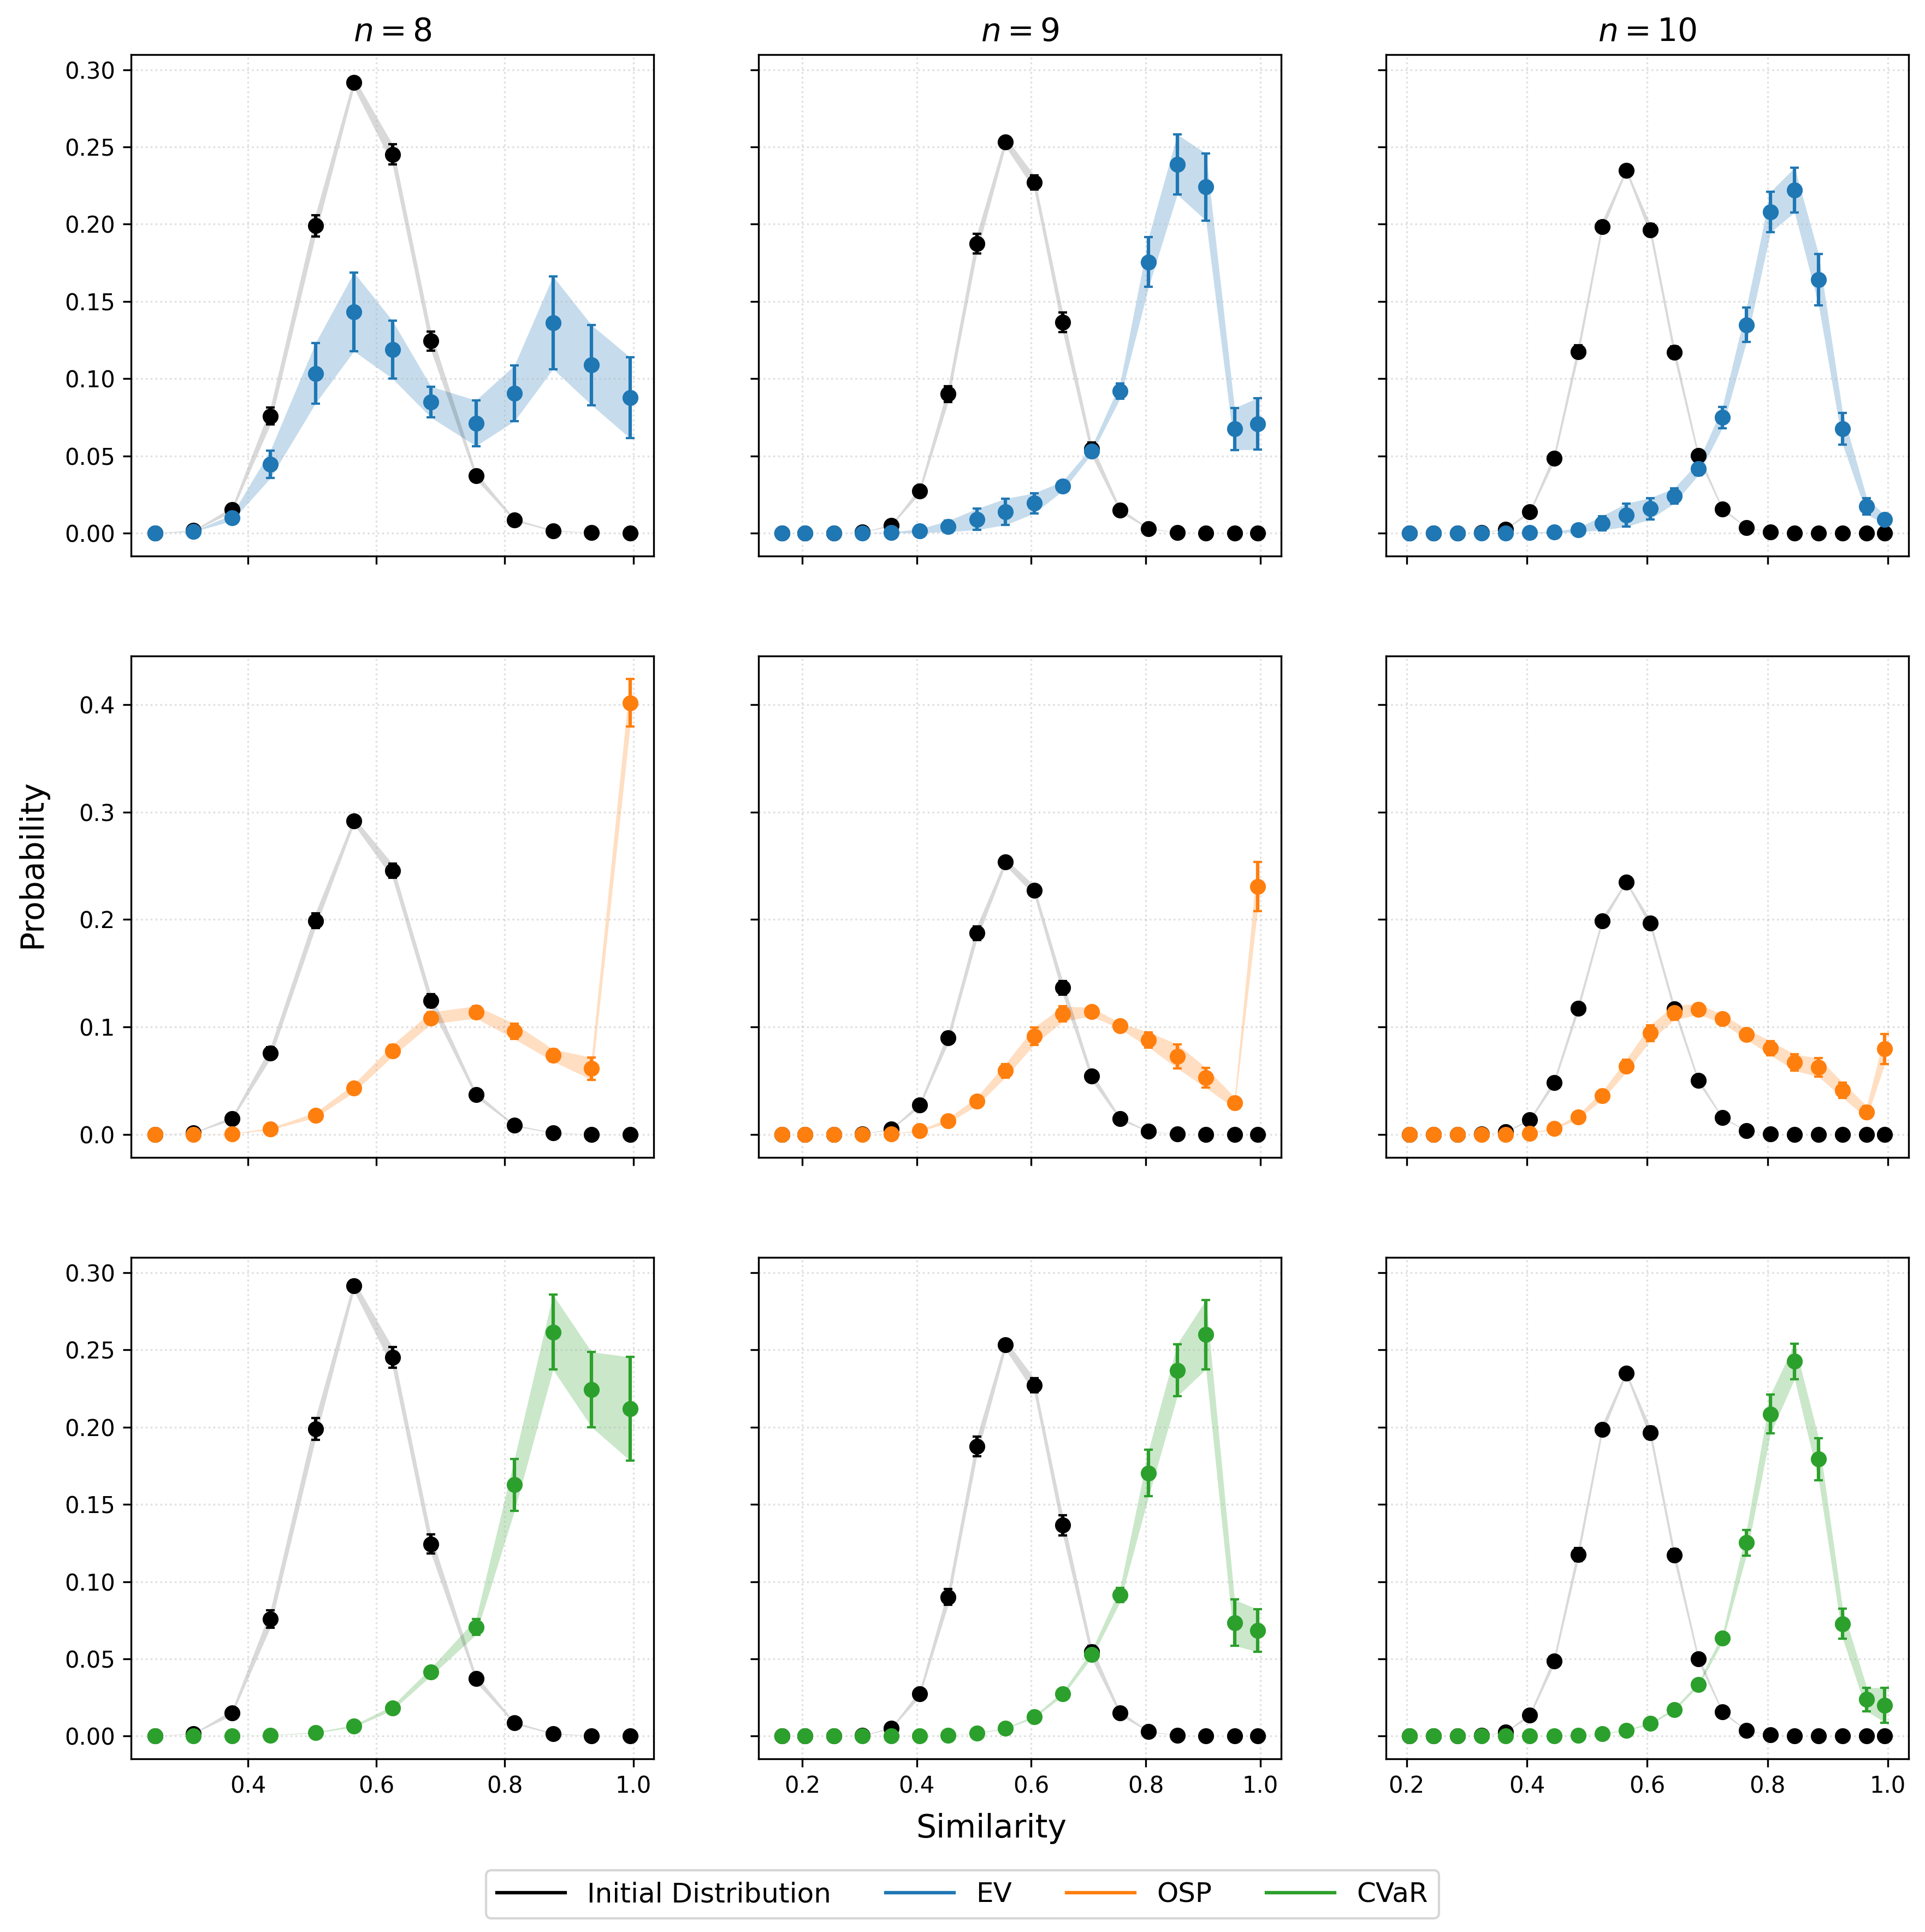
\includegraphics[width=\textwidth]{similarity_distributions_multiple.png} 
    \caption{Probability distributions for different objectives and sizes}
    \label{fig:similarity dist}
\end{figure}

\begin{figure}[htbp]
    \centering
    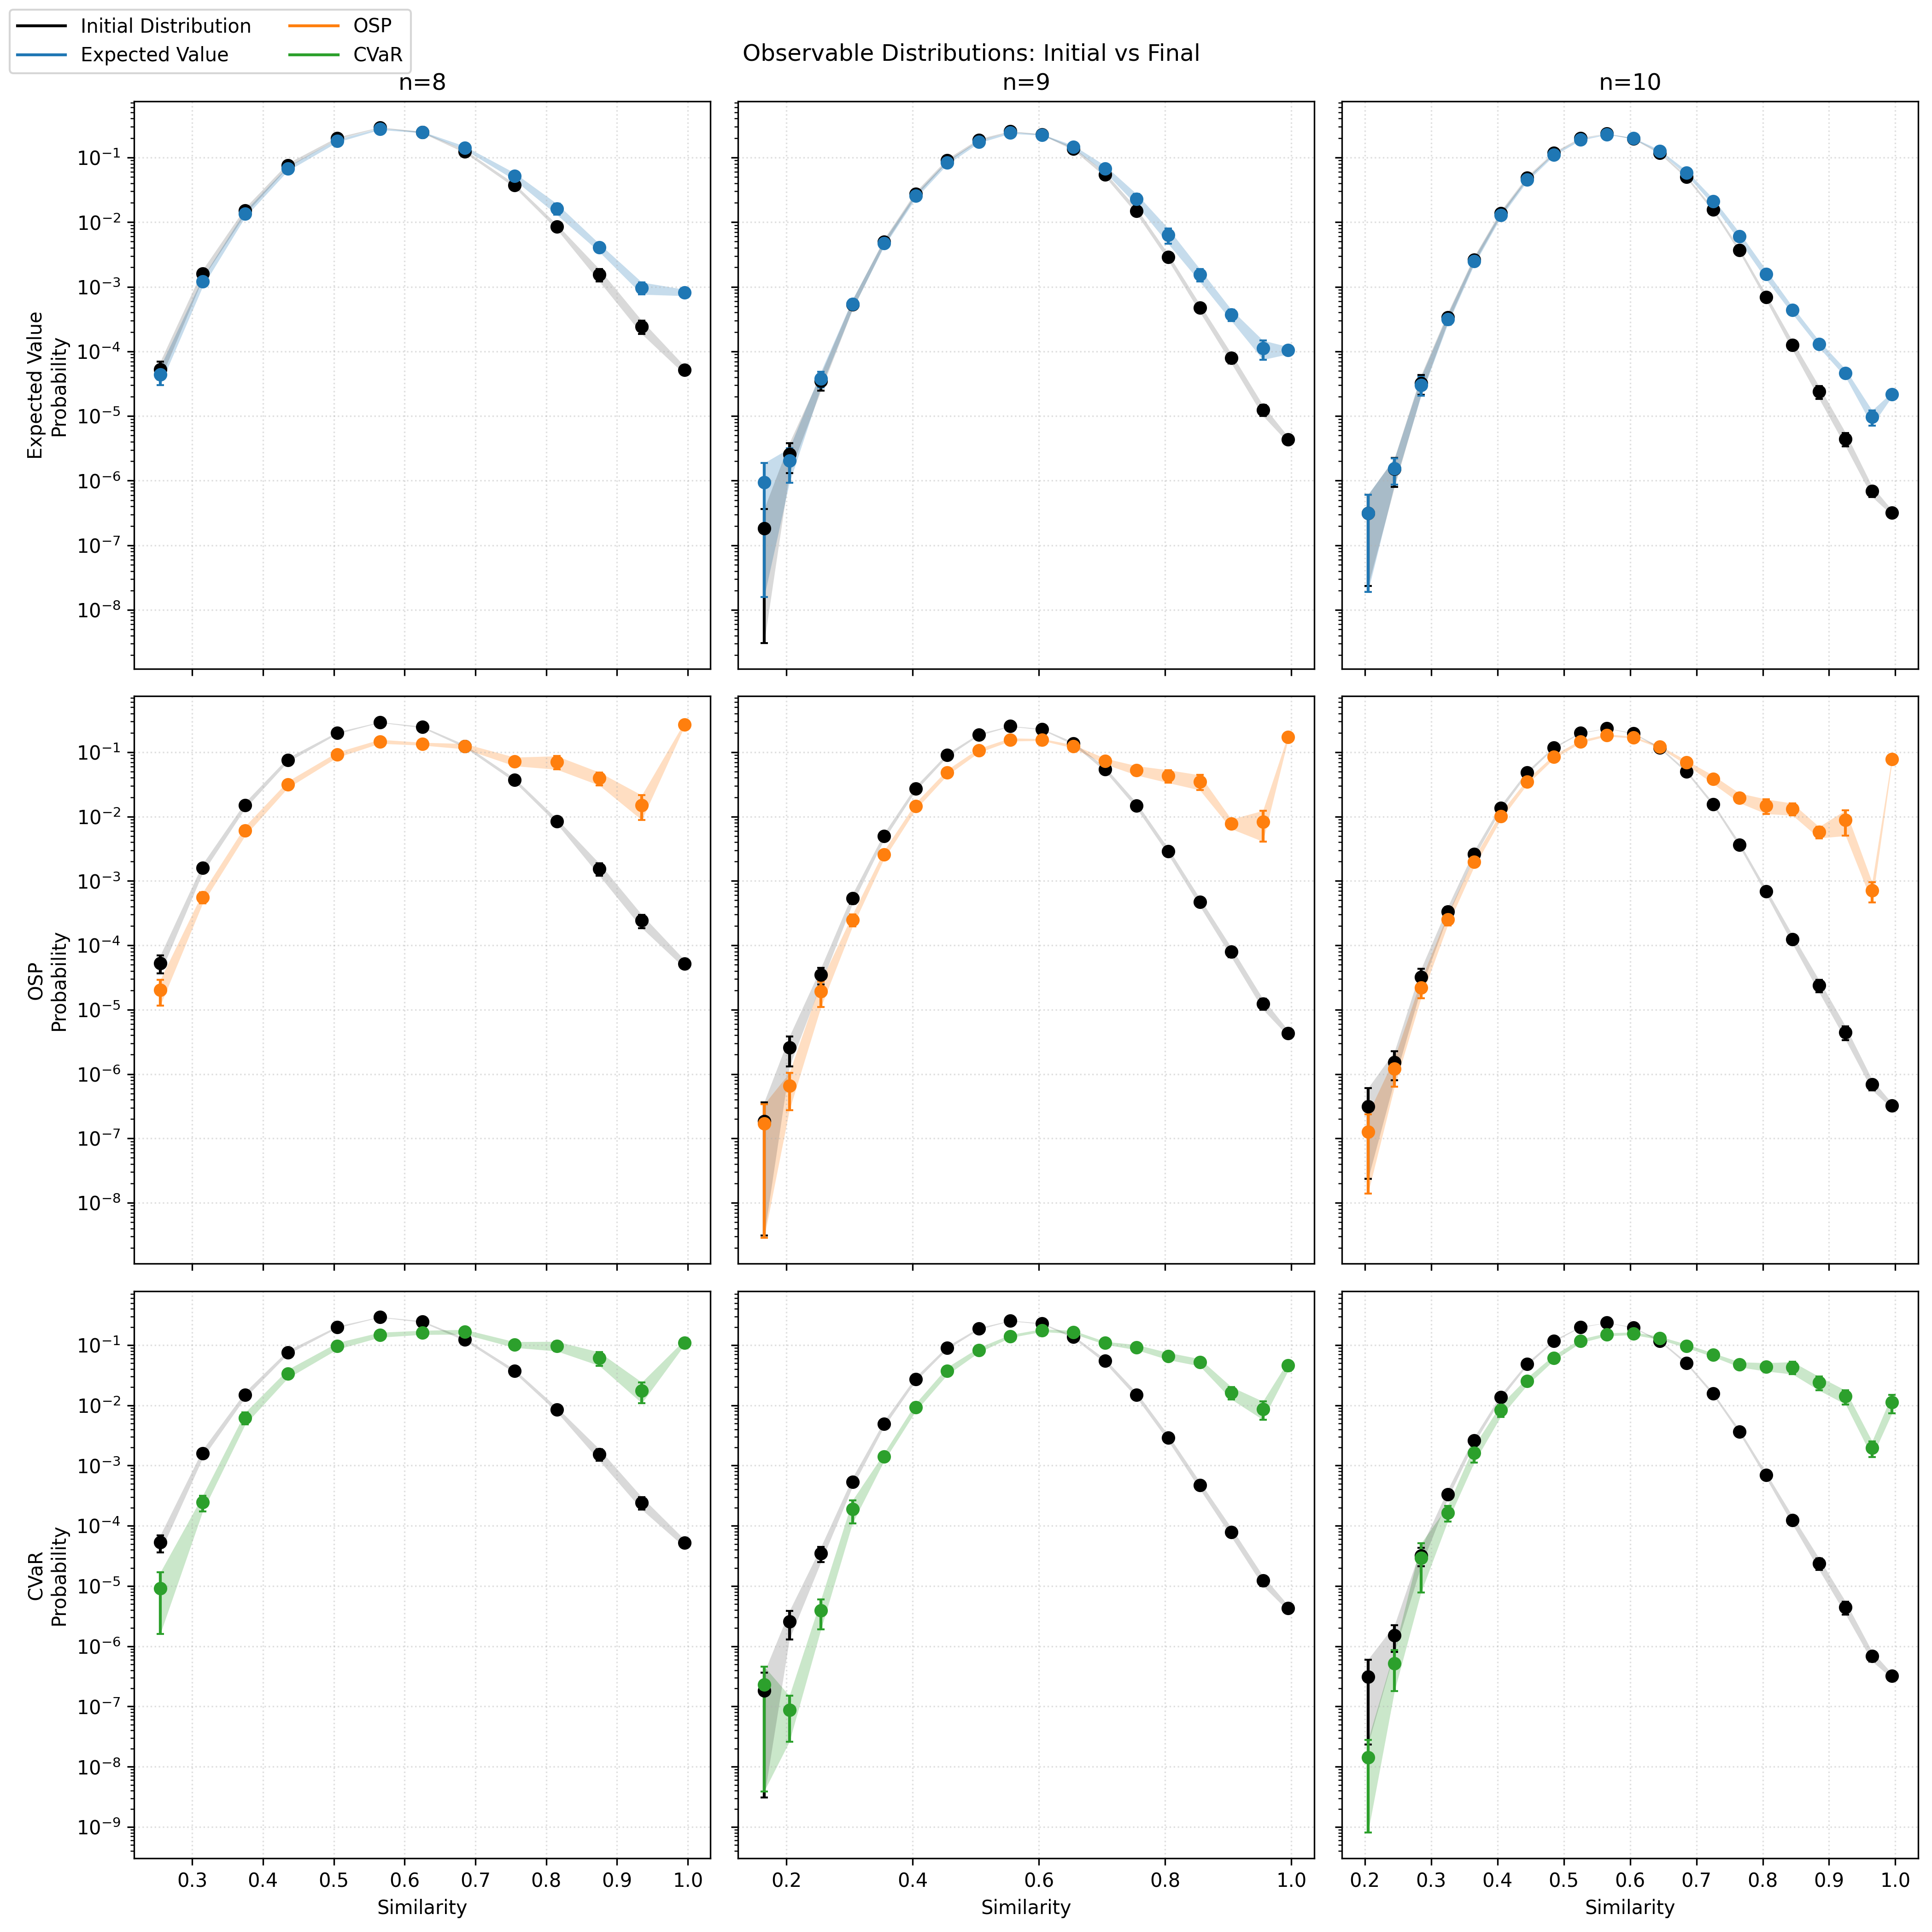
\includegraphics[width=\textwidth]{log_similarity_distributions_multiple.png} 
    \caption{Log probability distributions for different objectives and sizes}
    \label{fig:similarity log dist}
\end{figure}

Figure \ref{fig:osp} is a boxplot showing the probability of measuring the optimal solution (OSP) after amplification.
\begin{figure}[htbp]
    \centering
    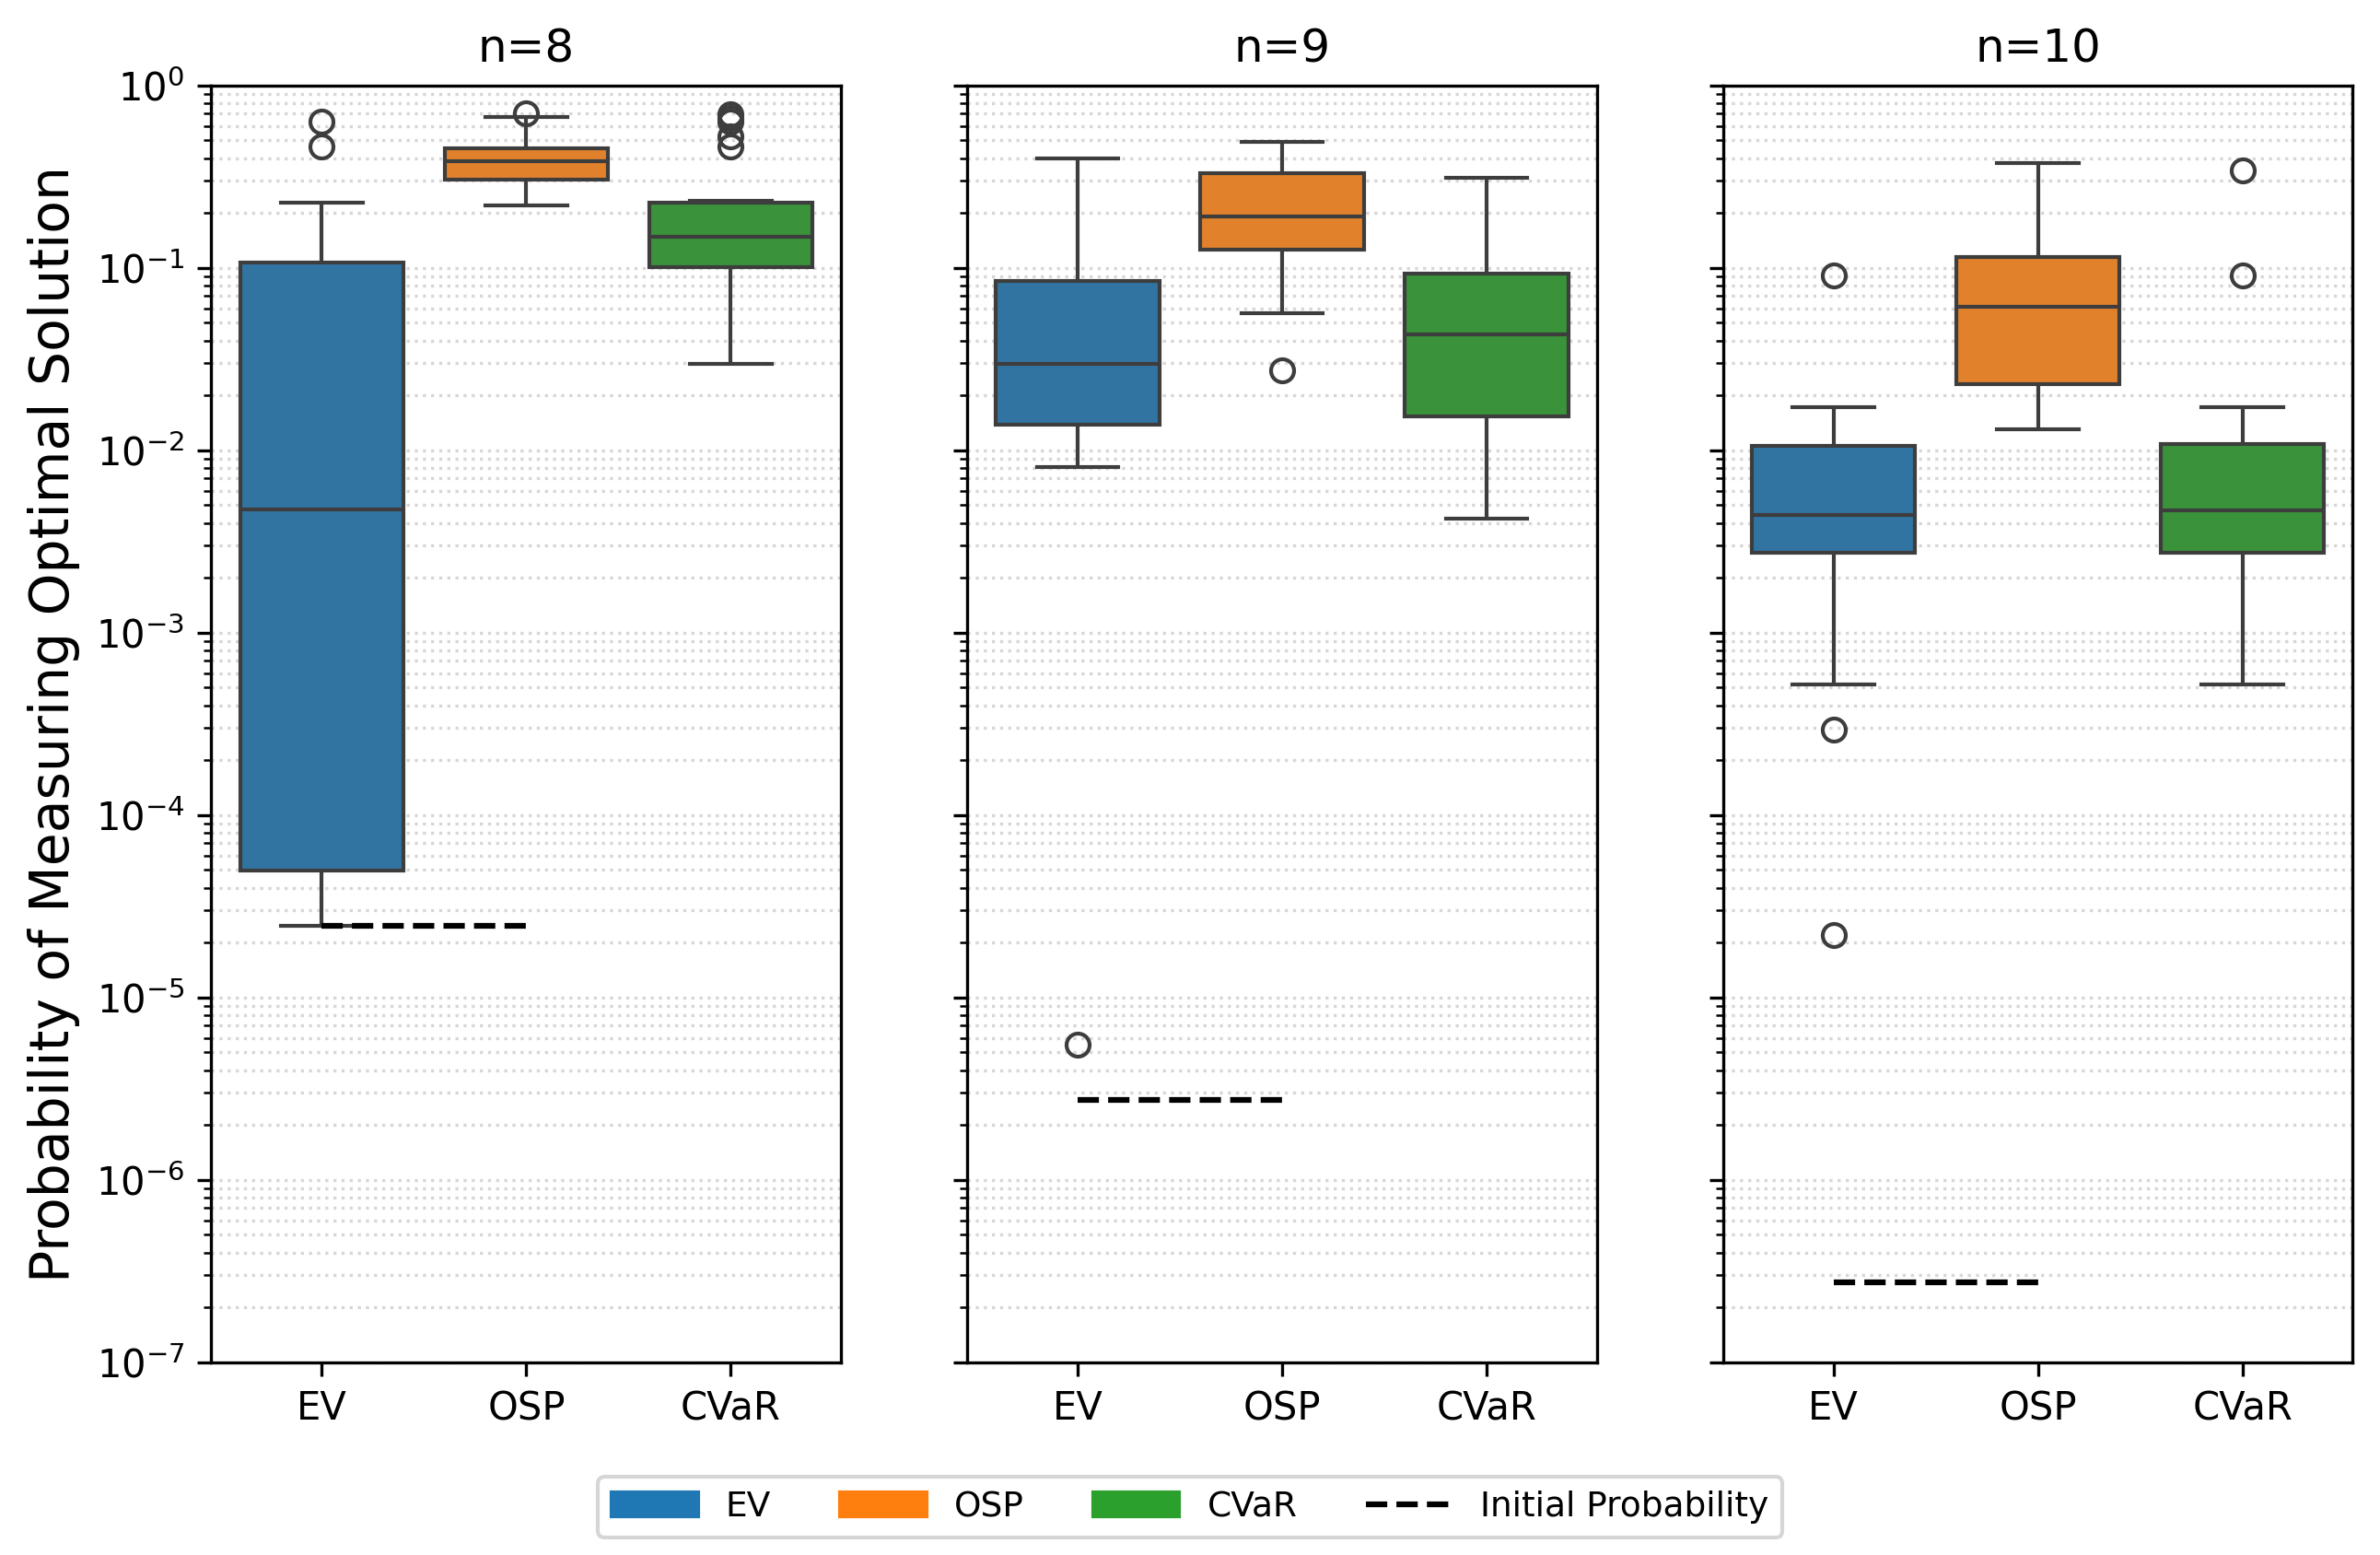
\includegraphics[width=\textwidth]{OSP_boxplot_multiple.png} 
    \caption{Optimal solution probability (OSP) distributions}
    \label{fig:osp}
\end{figure}



\section{Hamming Distance Analysis}

Figure \ref{fig:avg ham} shows the mean Hamming distance for each problem instance.
\begin{figure}[htbp]
     \centering
     \begin{subfigure}{0.45\textwidth}
         \centering
         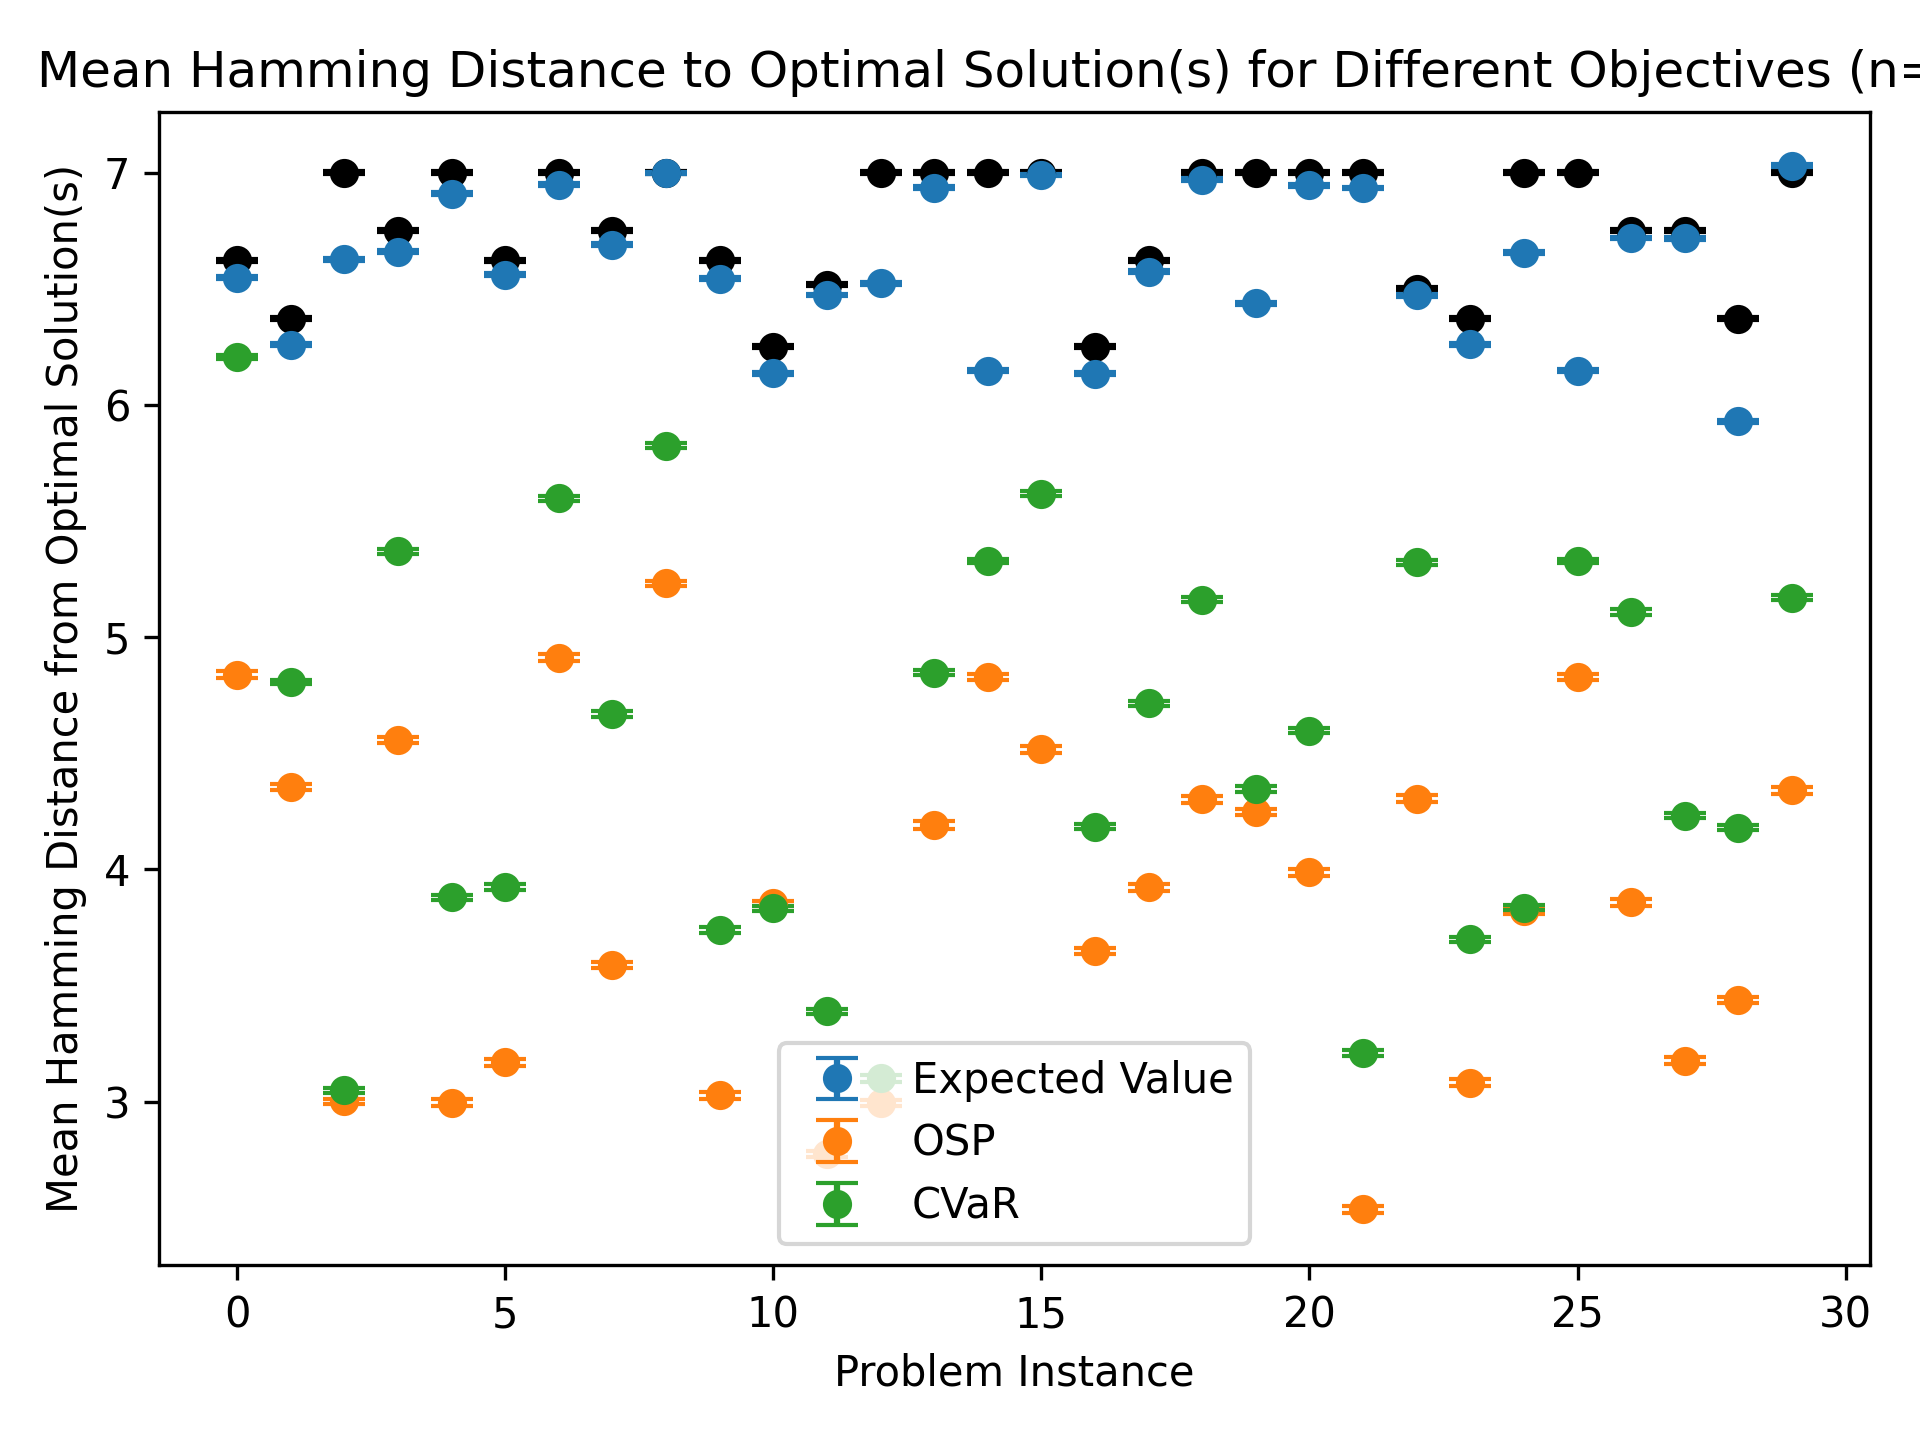
\includegraphics[width=\textwidth]{n=8_avg_hamming_distance_each_instance.png}
         \caption{$n=8$}
         \label{fig:avg ham 8}
     \end{subfigure}
     \hfill
     \begin{subfigure}{0.45\textwidth}
         \centering
         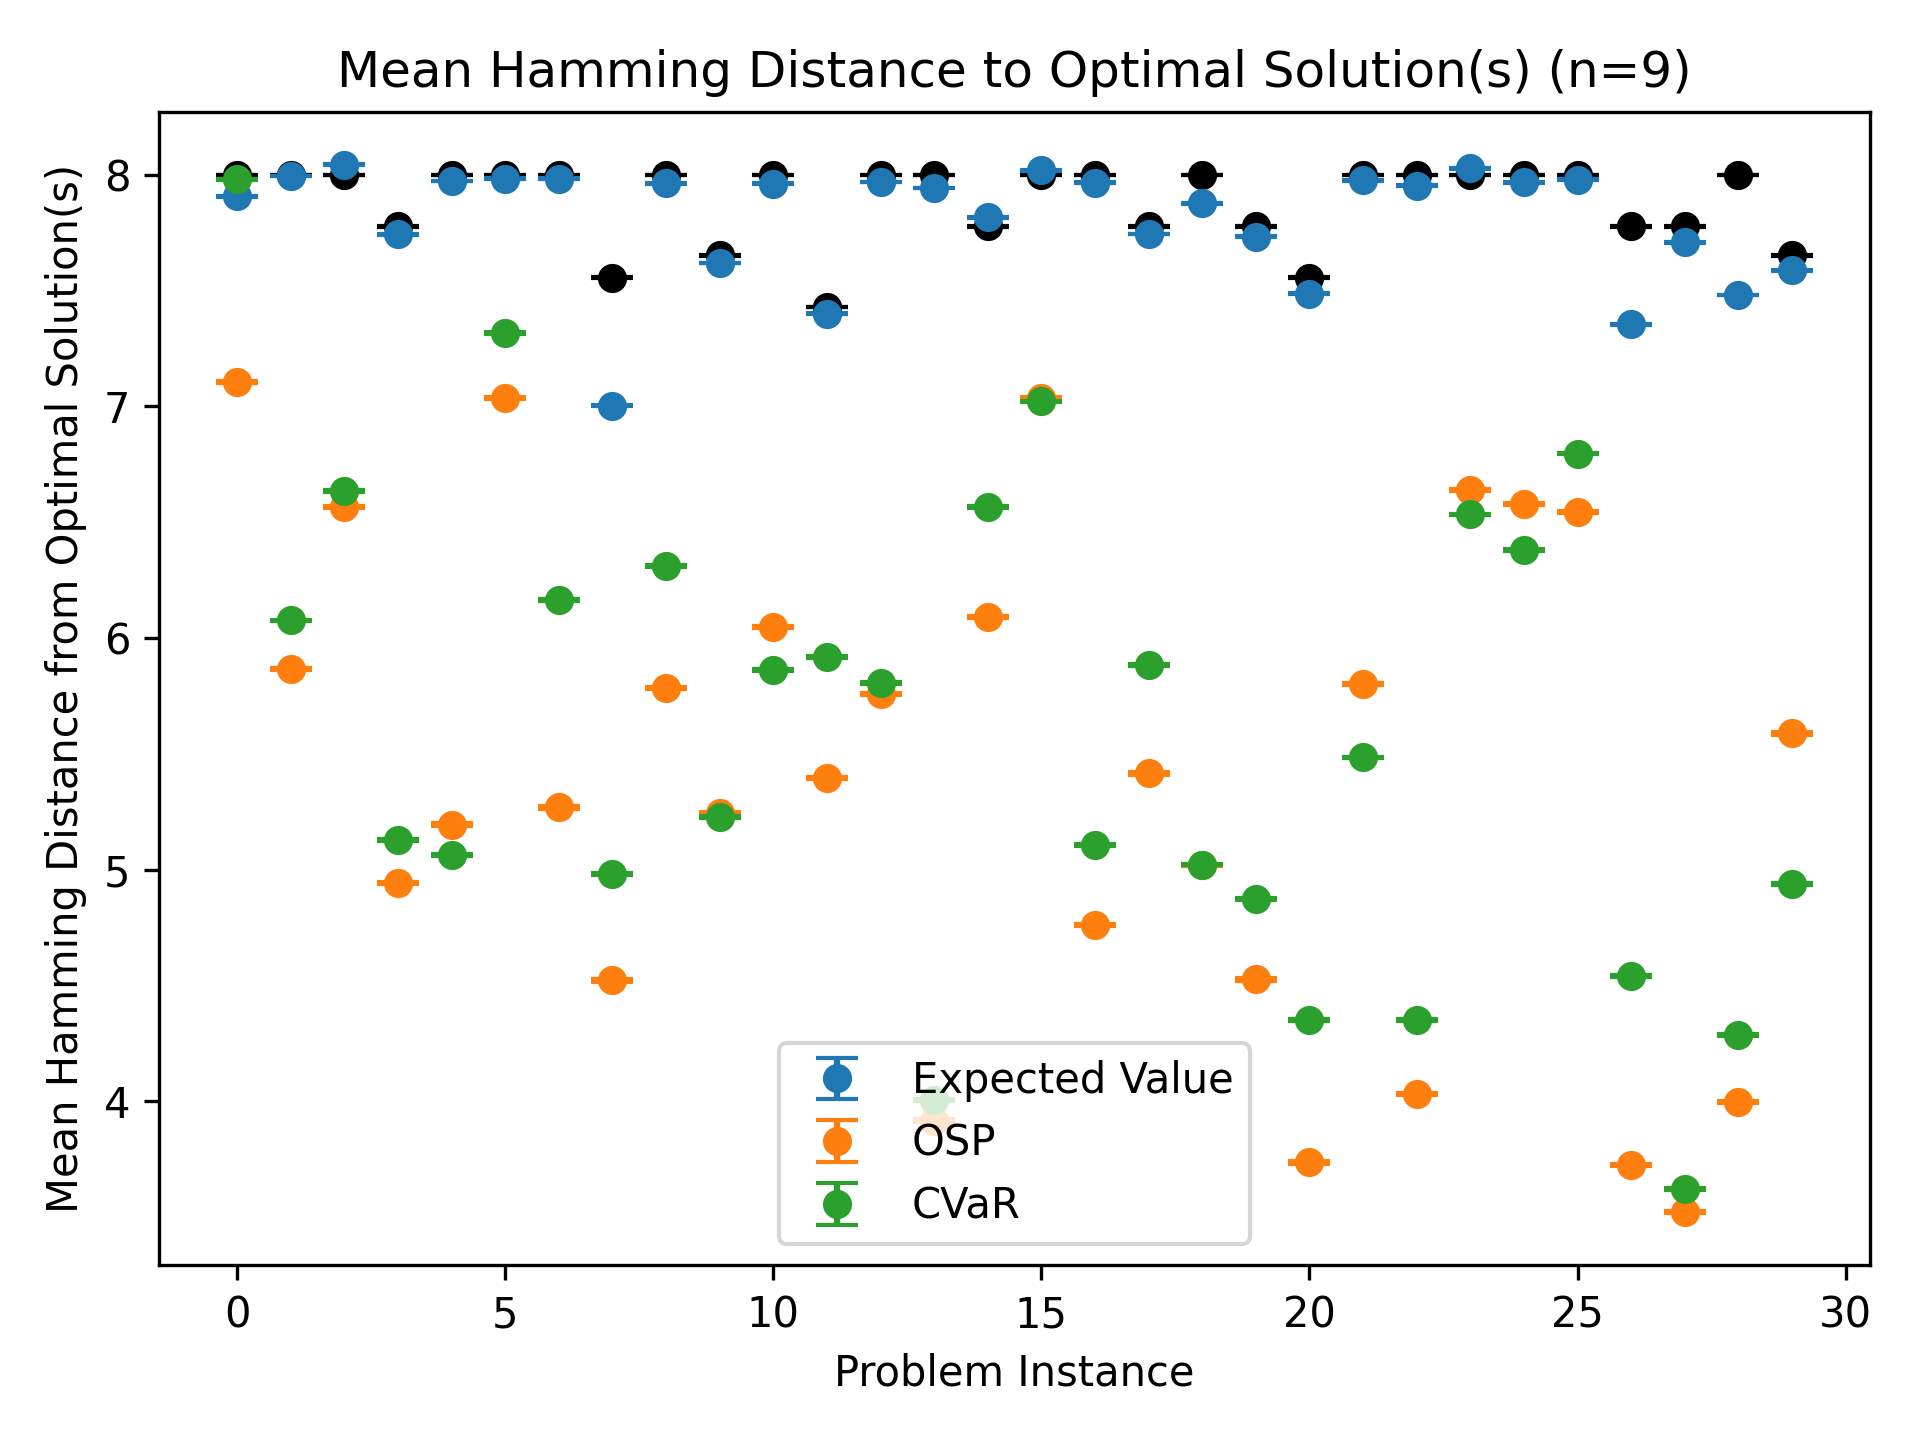
\includegraphics[width=\textwidth]{n=9_avg_hamming_distance_each_instance.png}
         \caption{$n=9$}
         \label{fig:avg ham 9}
     \end{subfigure}
     \hfill
     \begin{subfigure}{\textwidth}
         \centering
         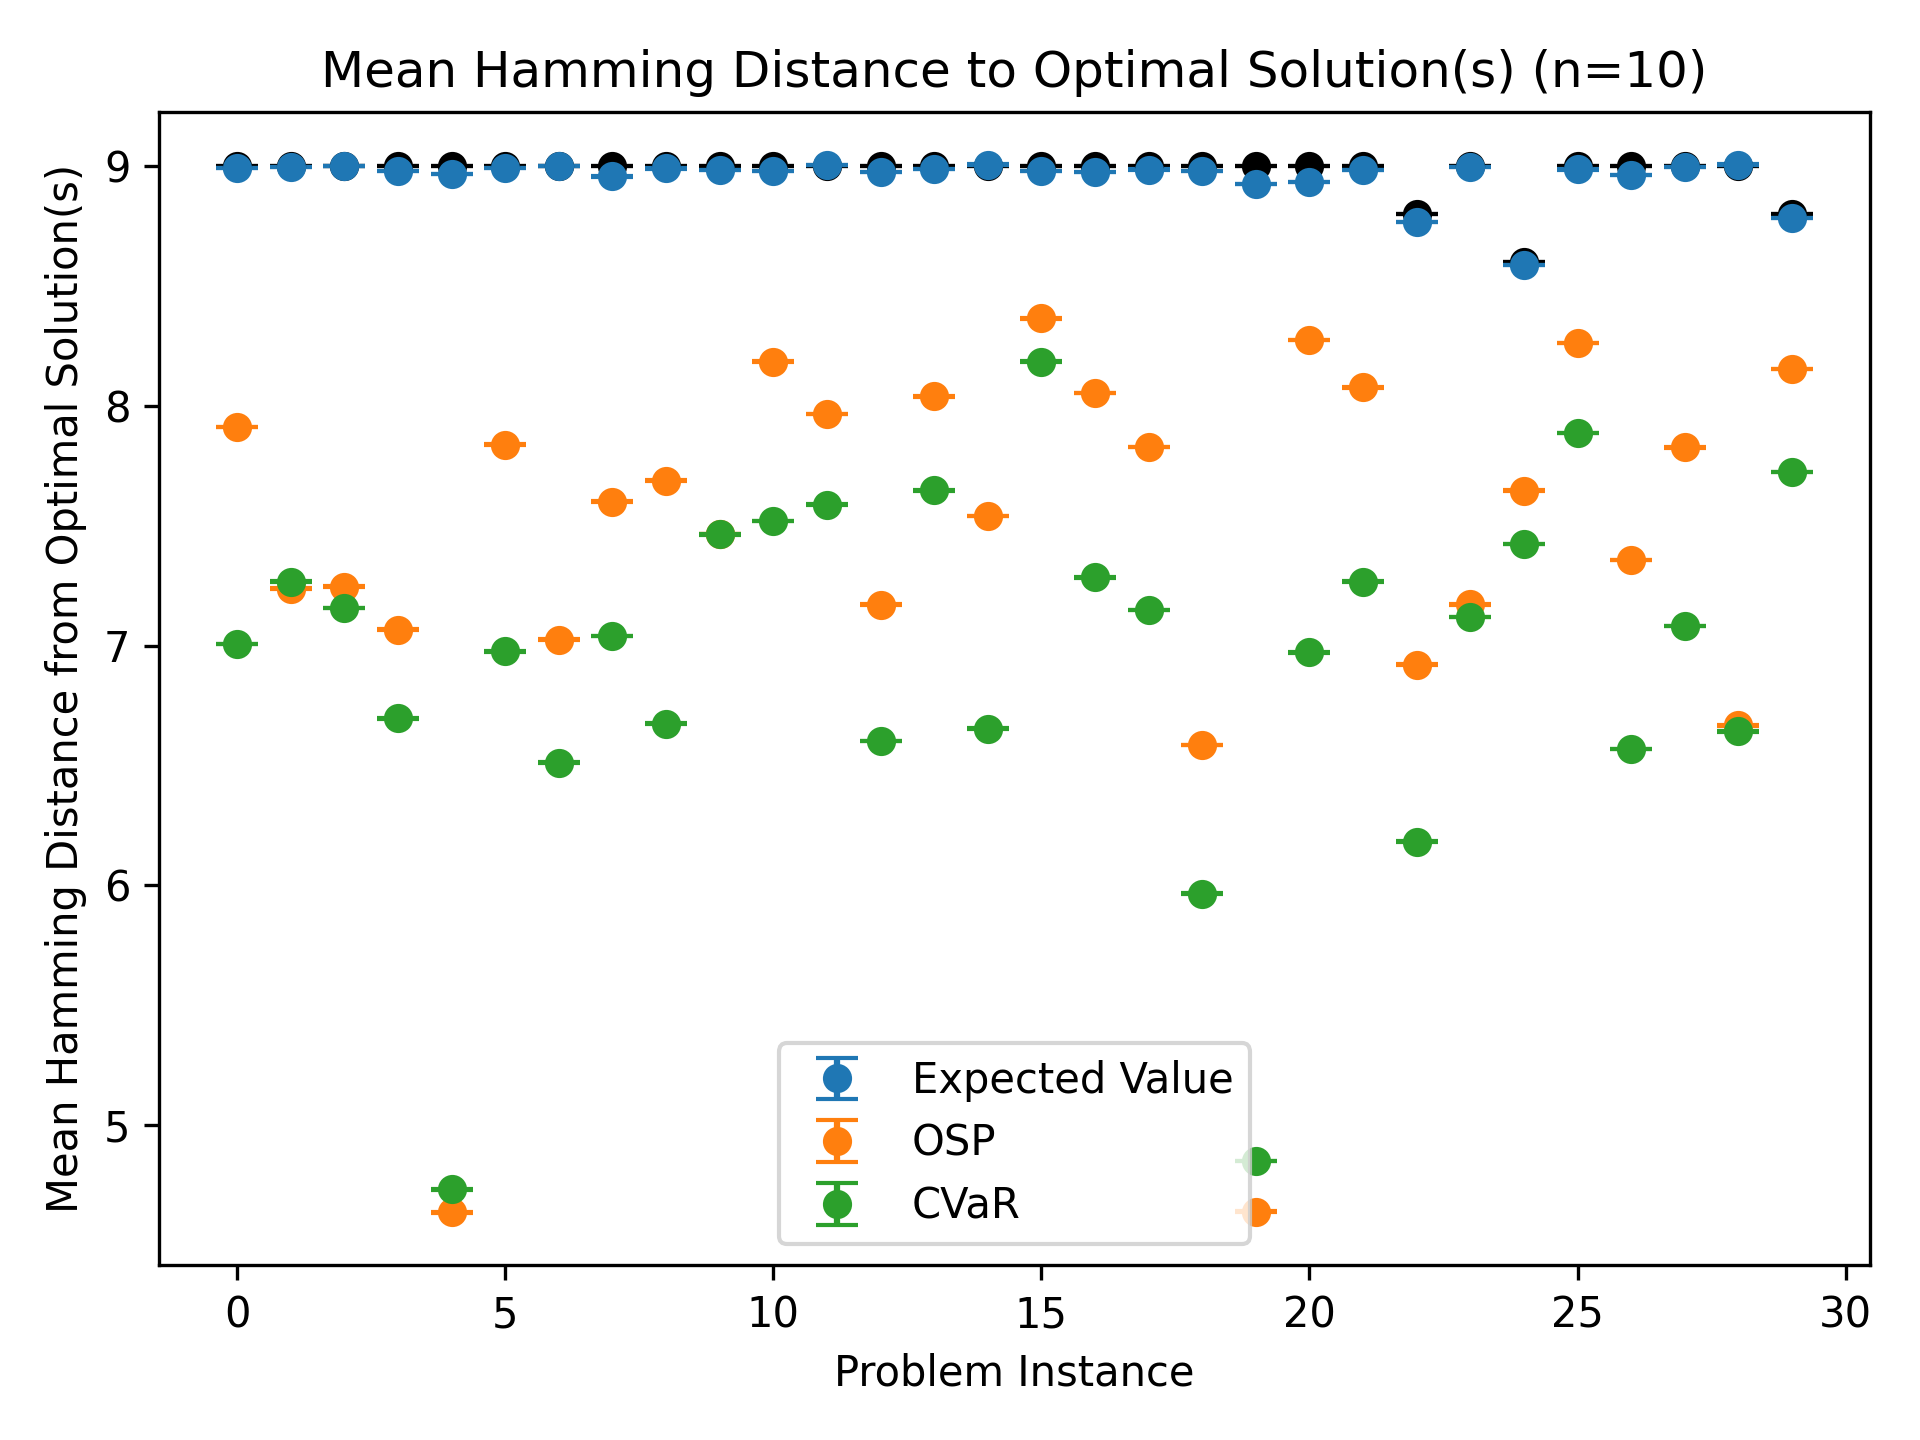
\includegraphics[width=\textwidth]{n=10_avg_hamming_distance_each_instance.png}
         \caption{$n=10$}
         \label{fig:avg ham 10}
     \end{subfigure}
        \caption{Mean hamming distance for each problem instance.}
        \label{fig:avg ham}
\end{figure}

Figure \ref{fig:ham improvement} shows the difference in Hamming distance between the initial distribution and after amplification.
\begin{figure}[htbp]
    \centering
    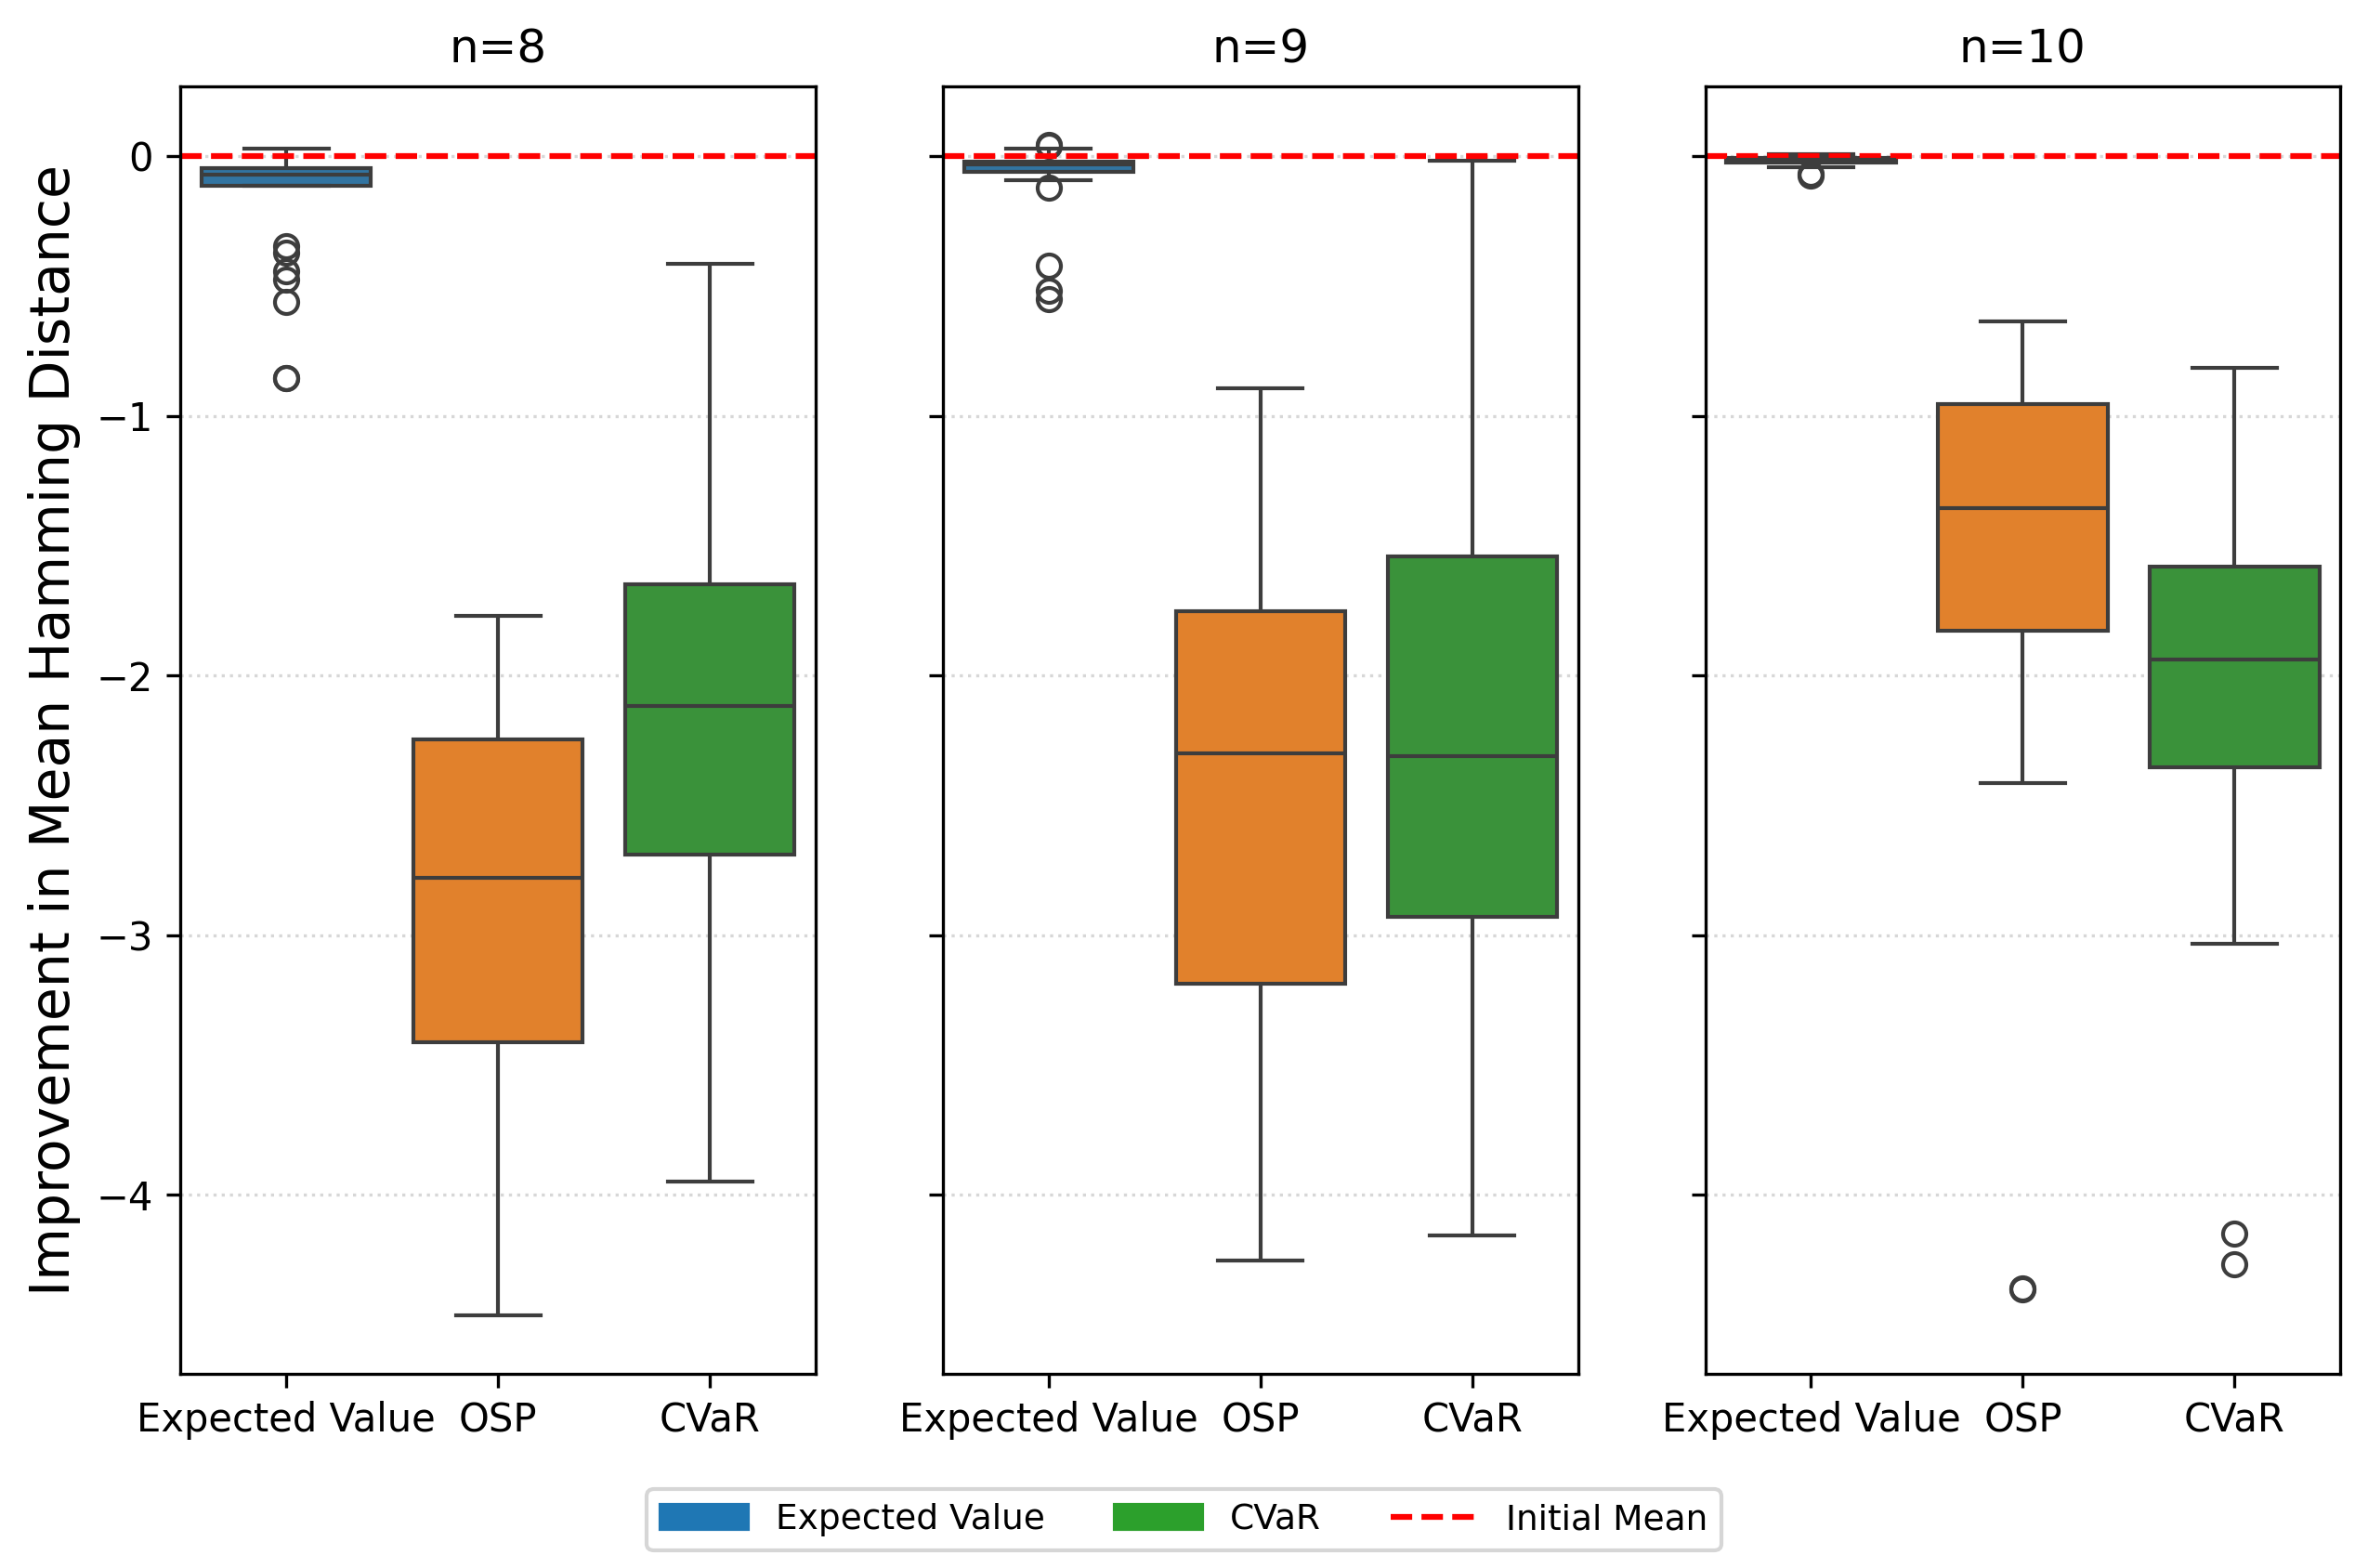
\includegraphics[width=\textwidth]{hamming_improvement_boxplot_multiple.png}
    \caption{Improvement in Hamming distance boxplot.}
    \label{fig:ham improvement}
\end{figure}

Figure \ref{fig:amp vs ham} shows how much amplification was applied to each solution based on their Hamming distance.
\begin{figure}[htbp]
    \centering
    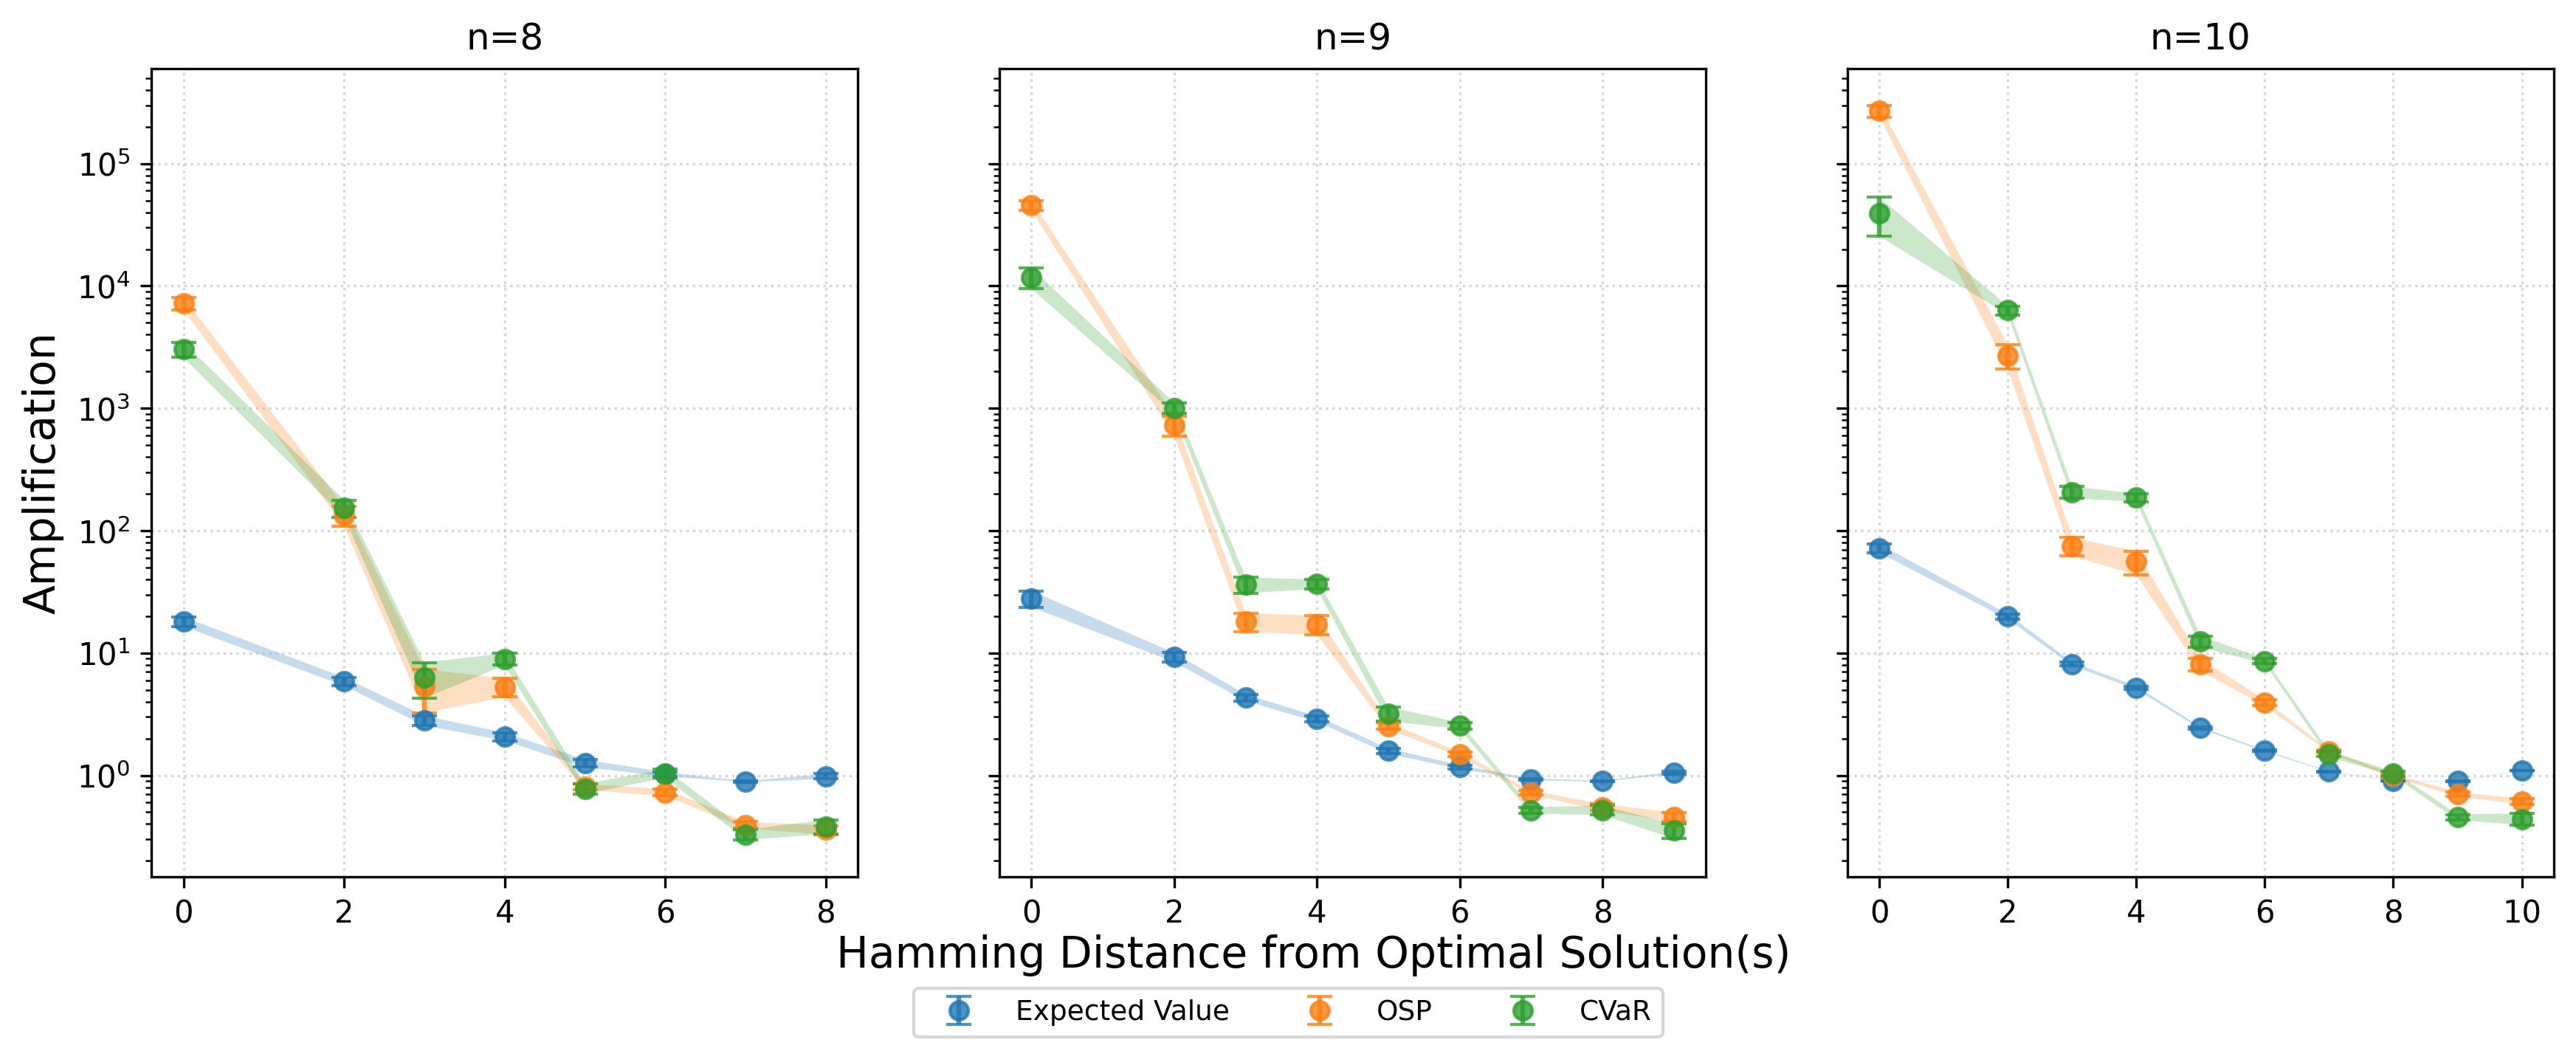
\includegraphics[width=\textwidth]{amplification_vs_hamming_multiple.png}
    \caption{Mean amplification applied to each solution grouped by their Hamming distance from the optimal solution.}
    \label{fig:amp vs ham}
\end{figure}



\section{Subshell Distance Analysis}

Figure \ref{fig:avg sub} depicts the average subshell distance before and after amplification for each problem instance.
\begin{figure}[htbp]
     \centering
     \begin{subfigure}{0.45\textwidth}
         \centering
         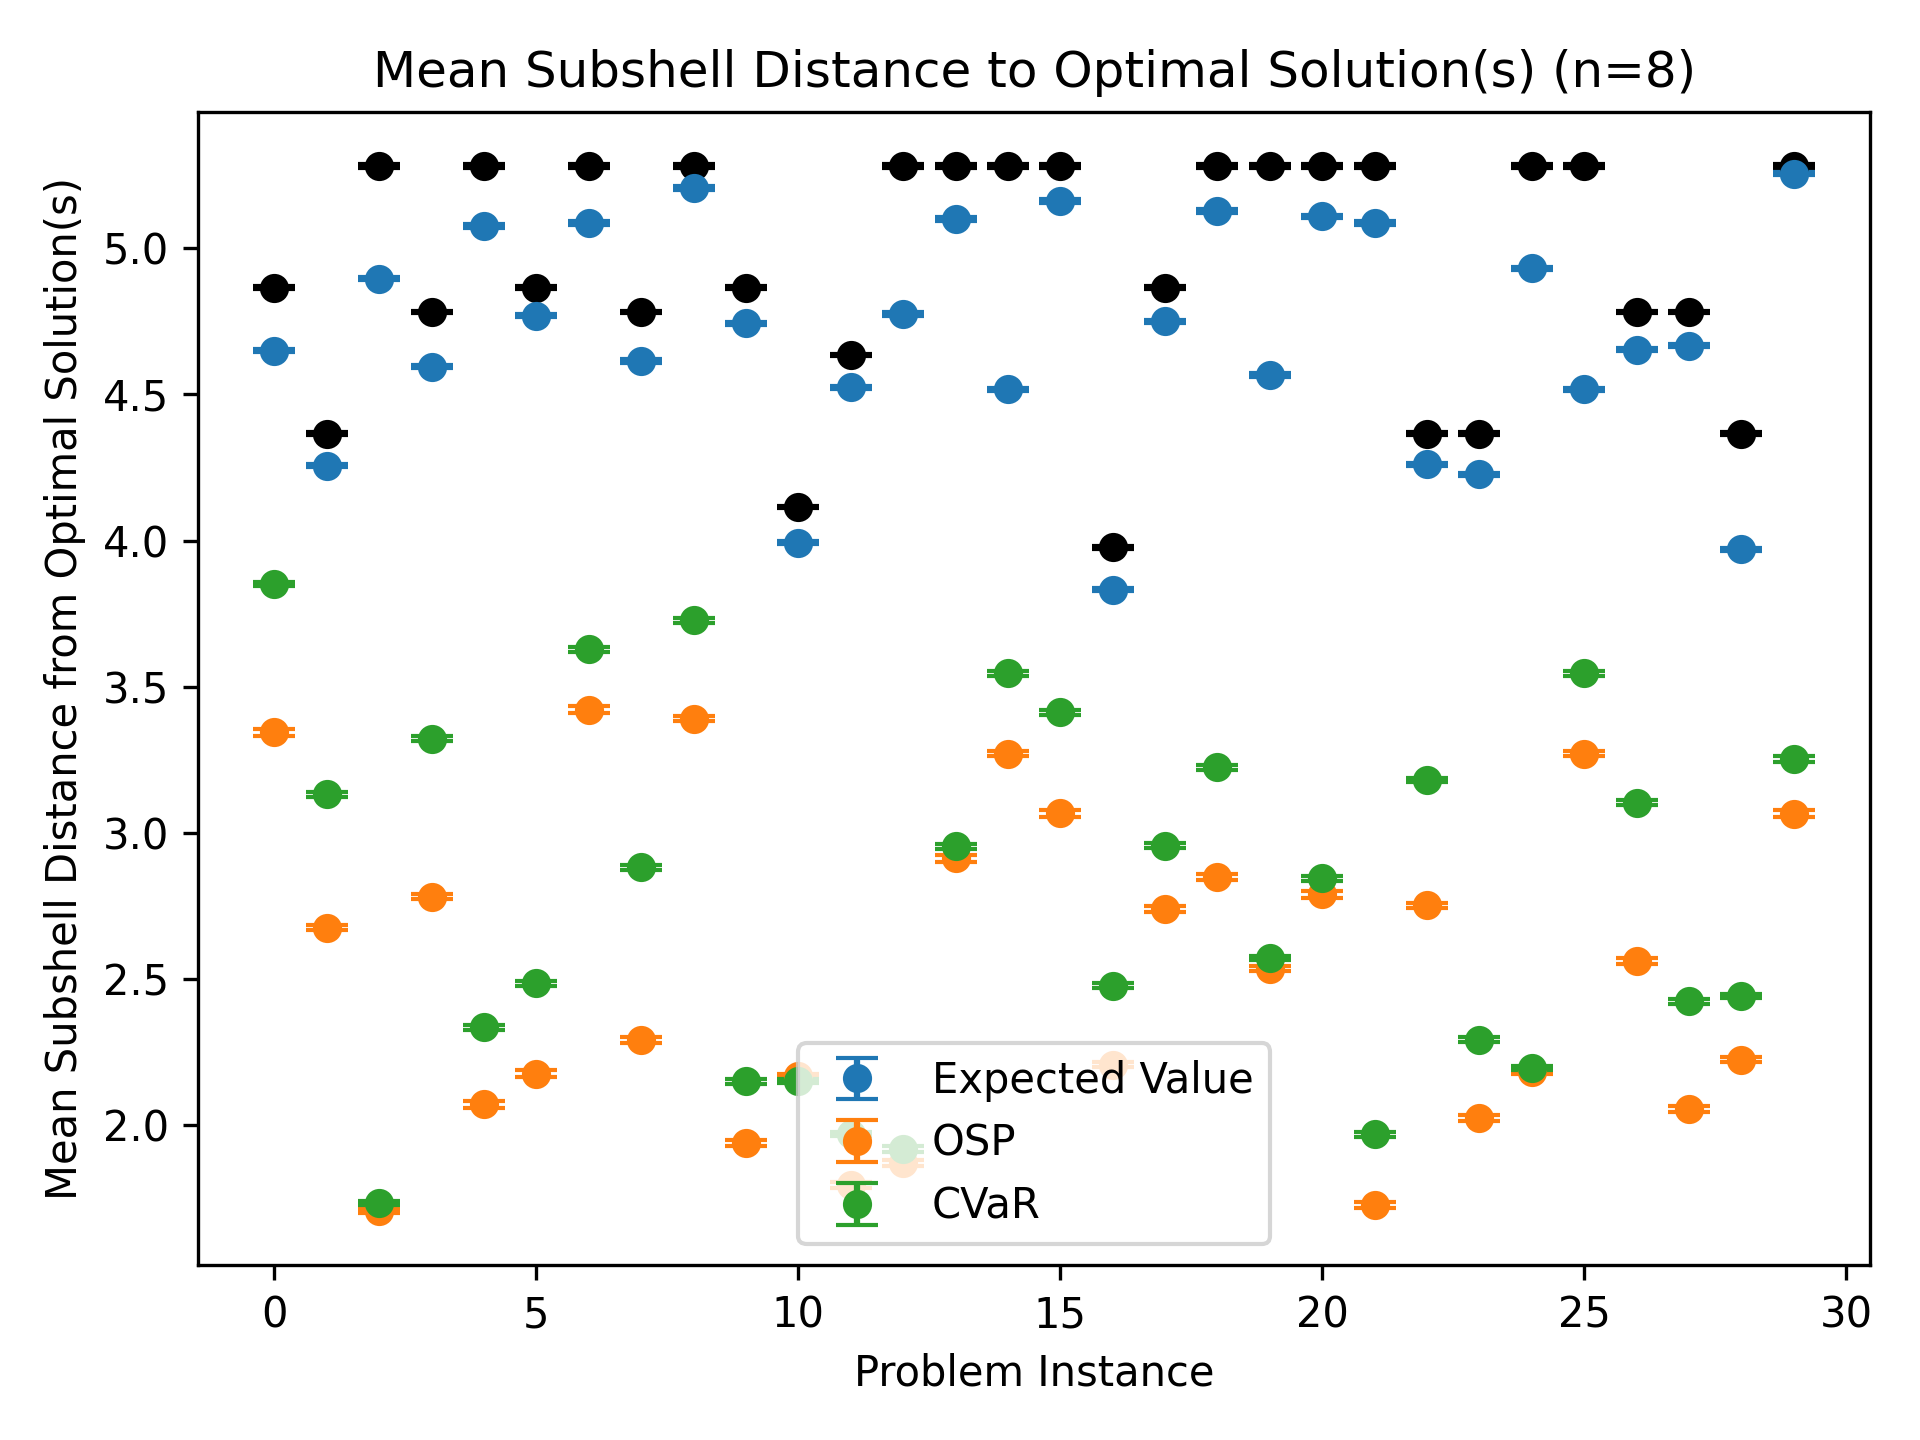
\includegraphics[width=\textwidth]{n=8_avg_subshell_distance_each_instance.png}
         \caption{$n=8$}
         \label{fig:avg sub 8}
     \end{subfigure}
     \hfill
     \begin{subfigure}{0.45\textwidth}
         \centering
         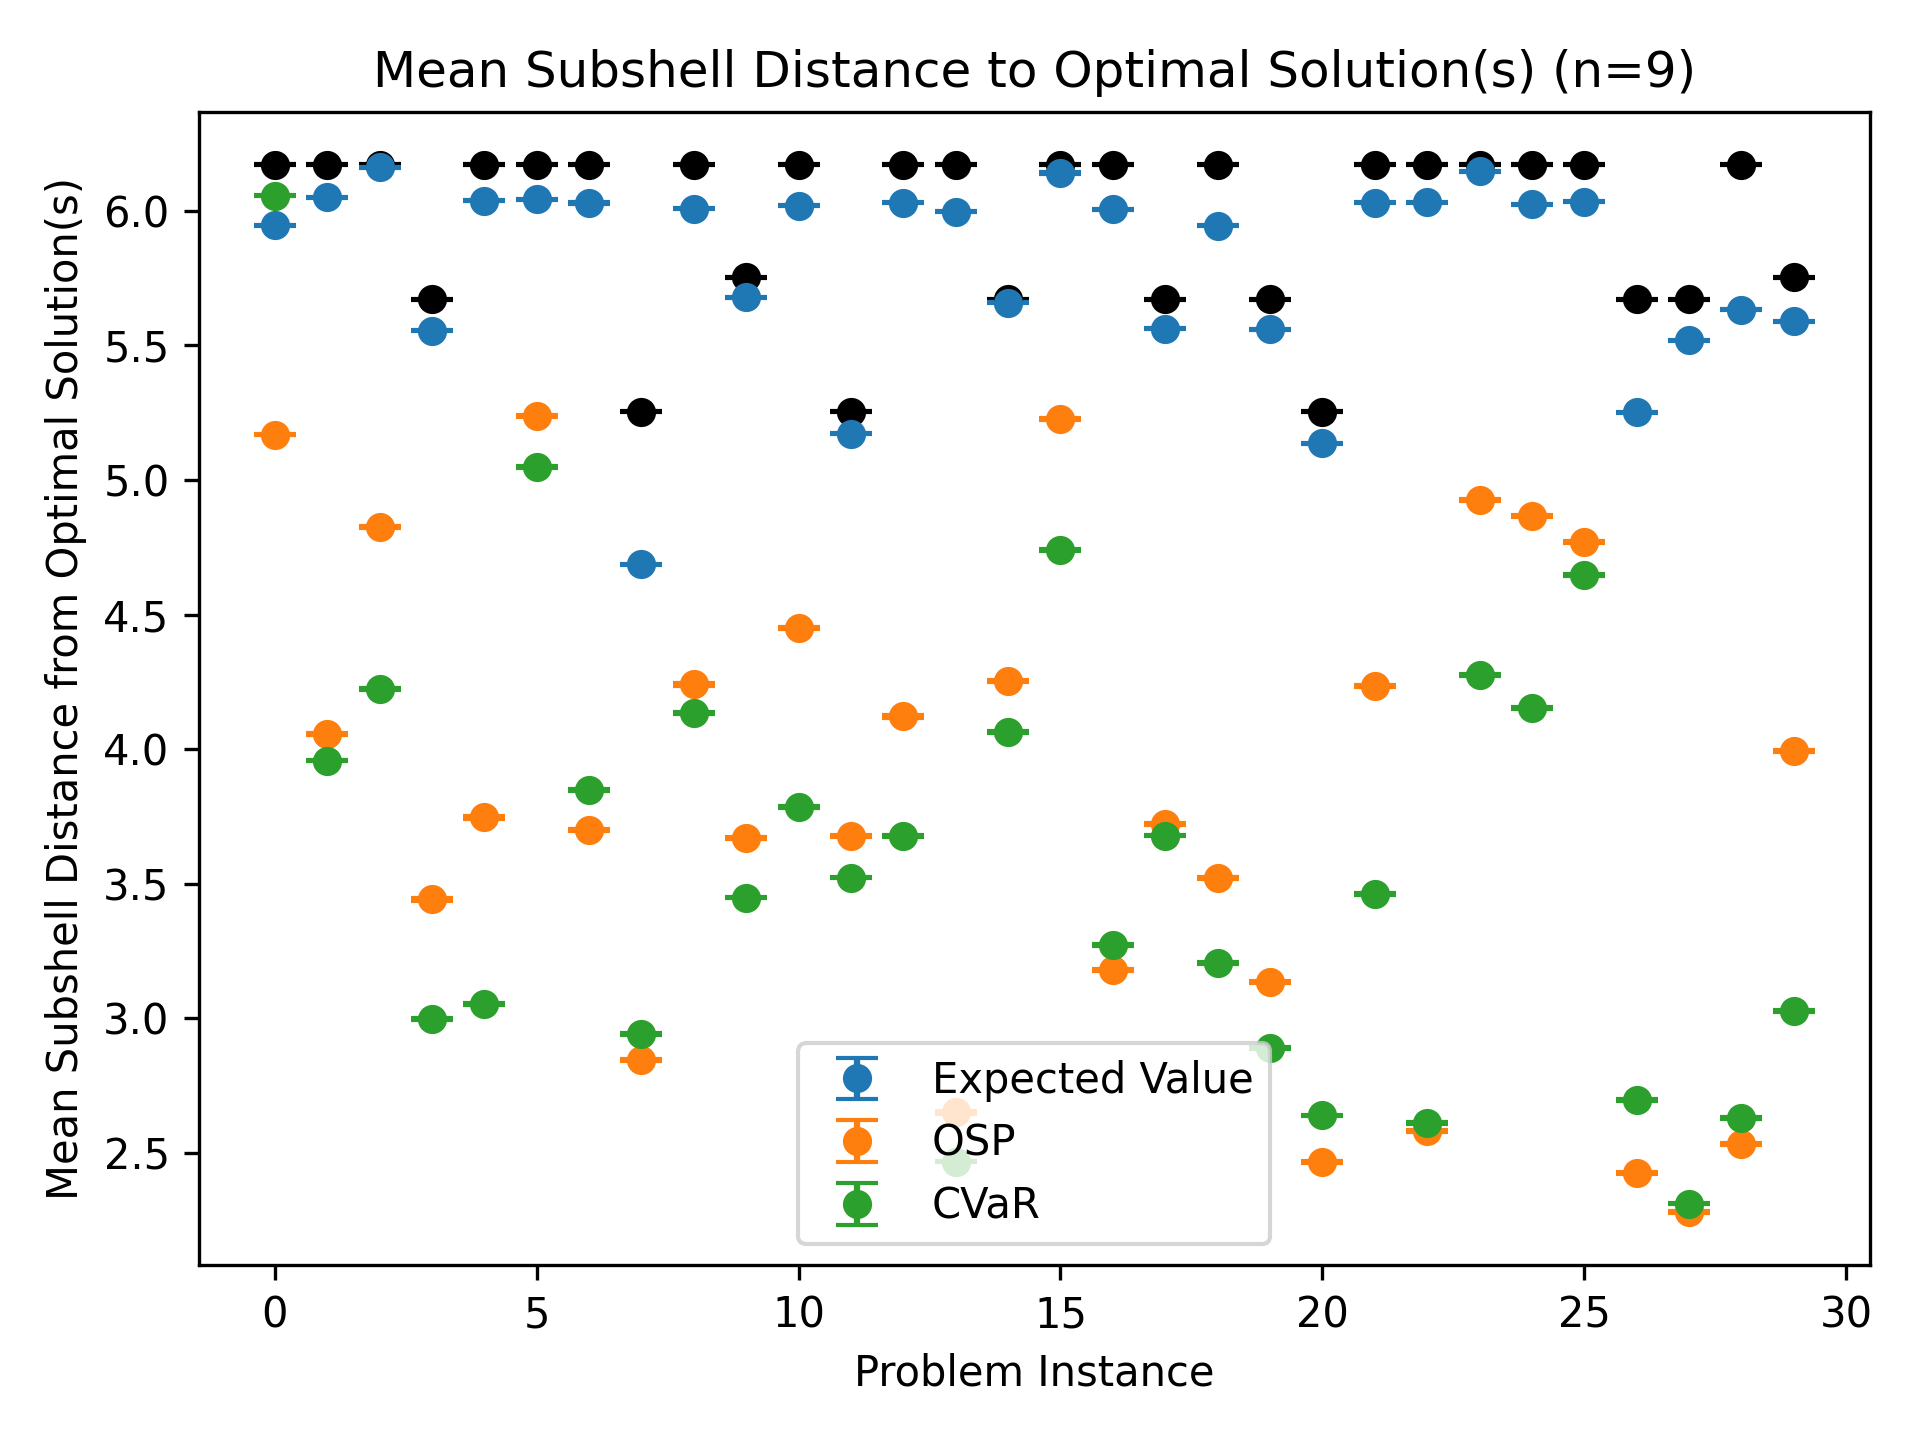
\includegraphics[width=\textwidth]{n=9_avg_subshell_distance_each_instance.png}
         \caption{$n=9$}
         \label{fig:avg sub 9}
     \end{subfigure}
     \hfill
     \begin{subfigure}{\textwidth}
         \centering
         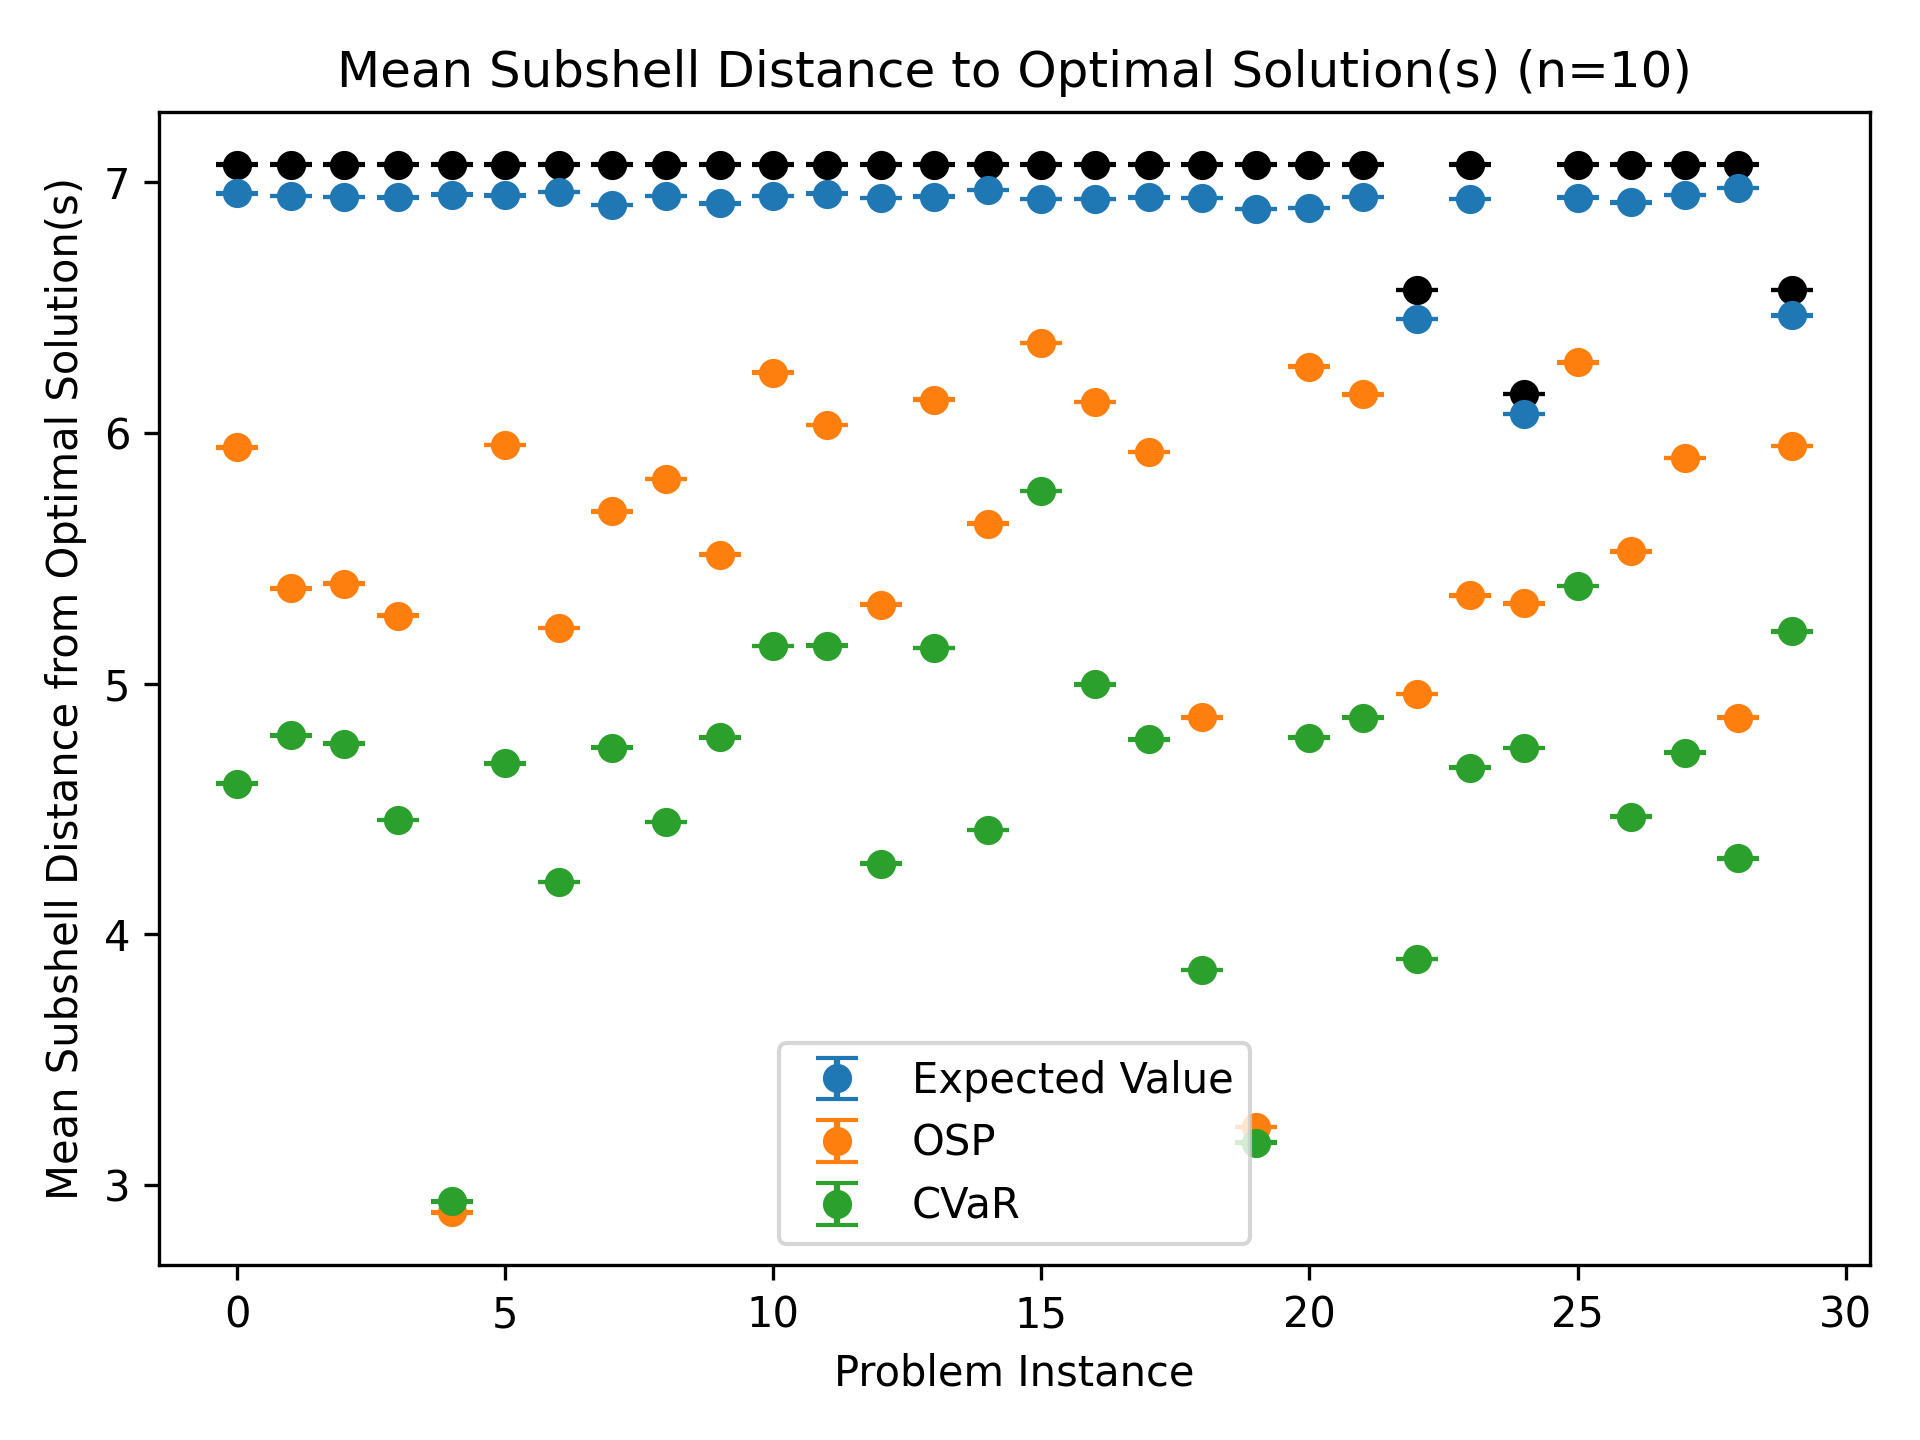
\includegraphics[width=\textwidth]{n=10_avg_subshell_distance_each_instance.png}
         \caption{$n=10$}
         \label{fig:avg sub 10}
     \end{subfigure}
        \caption{Mean subshell distance for each problem instance.}
        \label{fig:avg sub}
\end{figure}

Figure \ref{fig:sub improvement} shows the difference in mean subshell distance after amplification.
\begin{figure}[htbp]
    \centering
    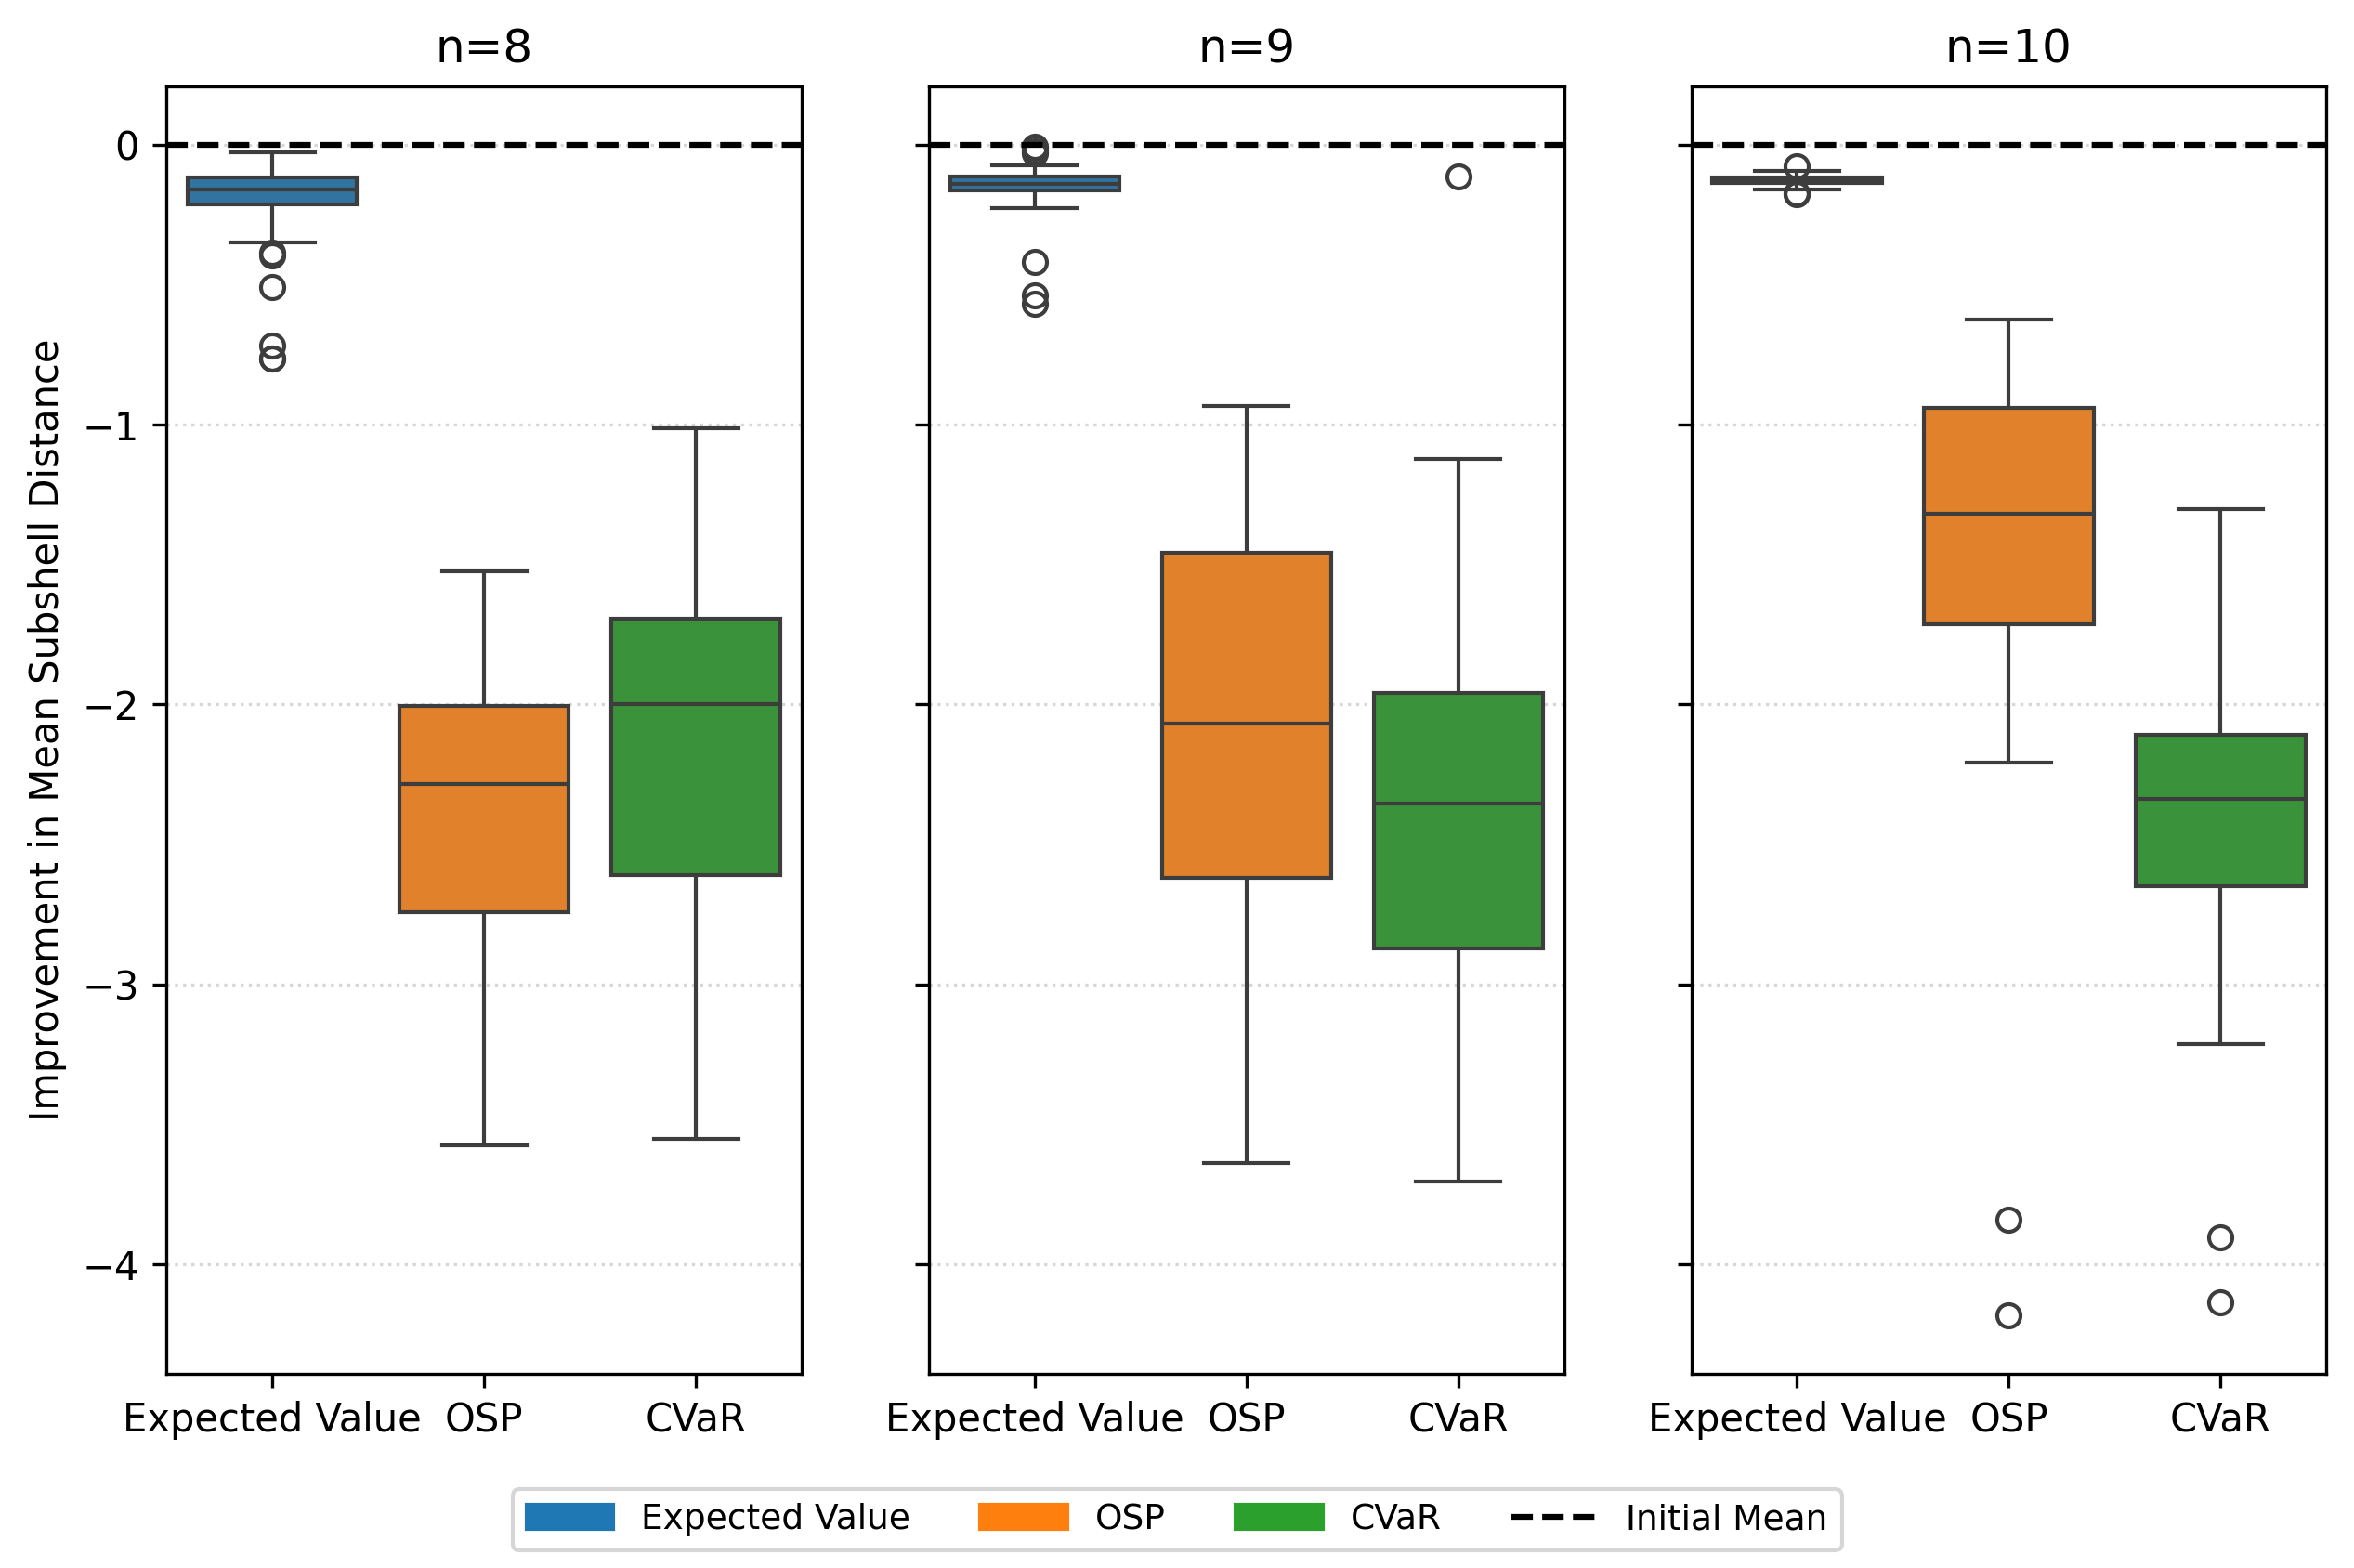
\includegraphics[width=\textwidth]{subshell_improvement_boxplot_multiple.png}
    \caption{Improvement in subshell distance boxplot.}
    \label{fig:sub improvement}
\end{figure}

Figure \ref{fig:amp vs sub} shows how much amplification was applied to each solution based on their subshell distance.
\begin{figure}[htbp]
    \centering
    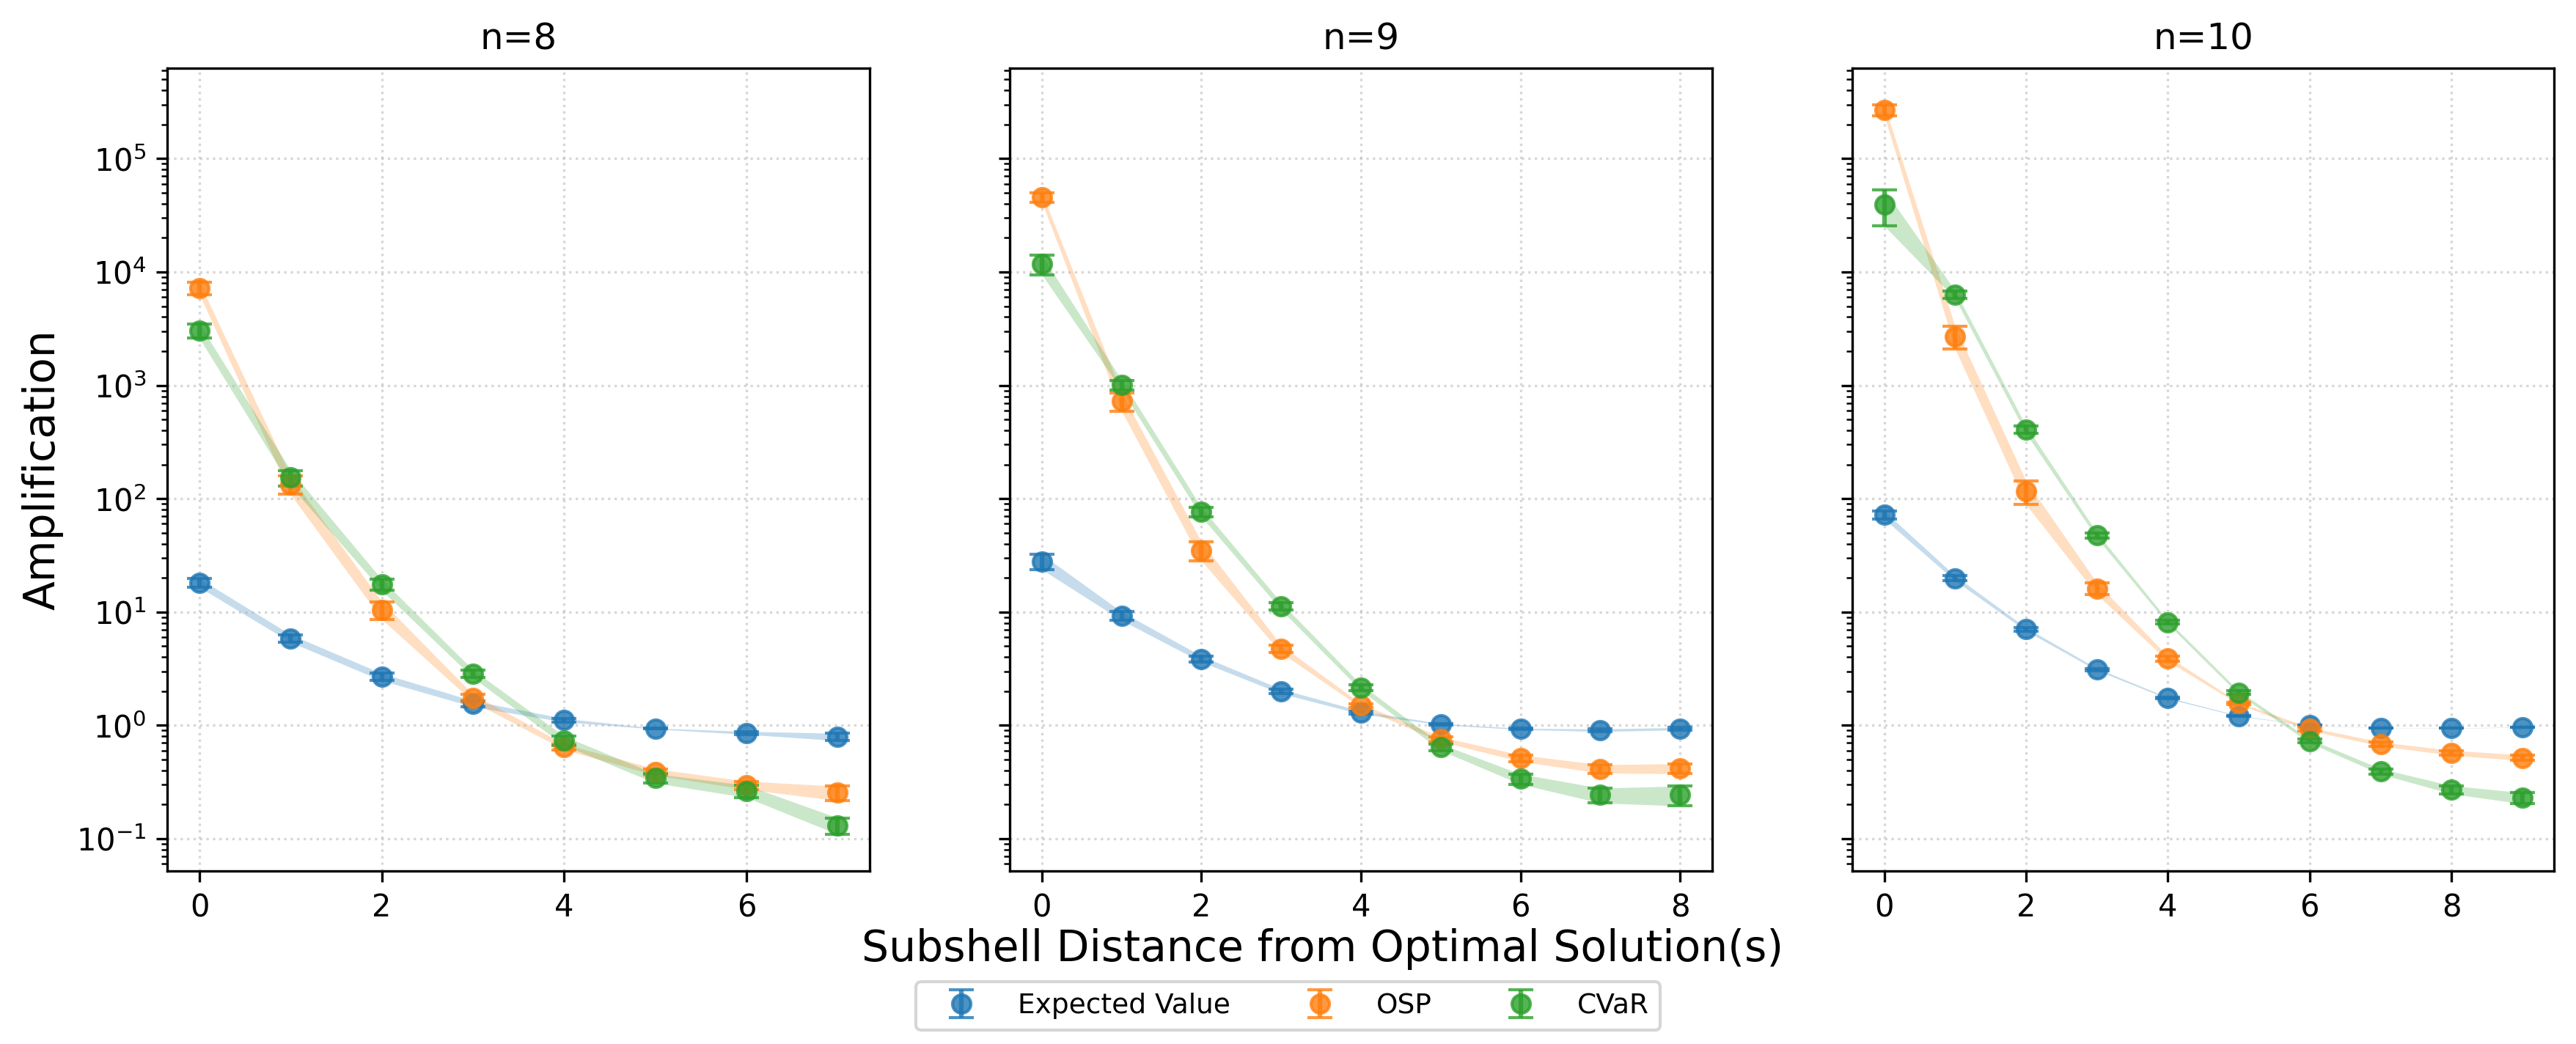
\includegraphics[width=\textwidth]{amplification_vs_subshell_multiple.png}
    \caption{Mean amplification applied to each solution grouped by their subshell distance from the optimal solution.}
    \label{fig:amp vs sub}
\end{figure}

Figure \ref{fig:mqg} shows the mean quality gap between the optimal solutions and the subshells. Mention accounting for cases with $n-2$ possible shell distances. And the fact that being monotonically increasing is a good thing.
\begin{figure}[htbp]
    \centering
    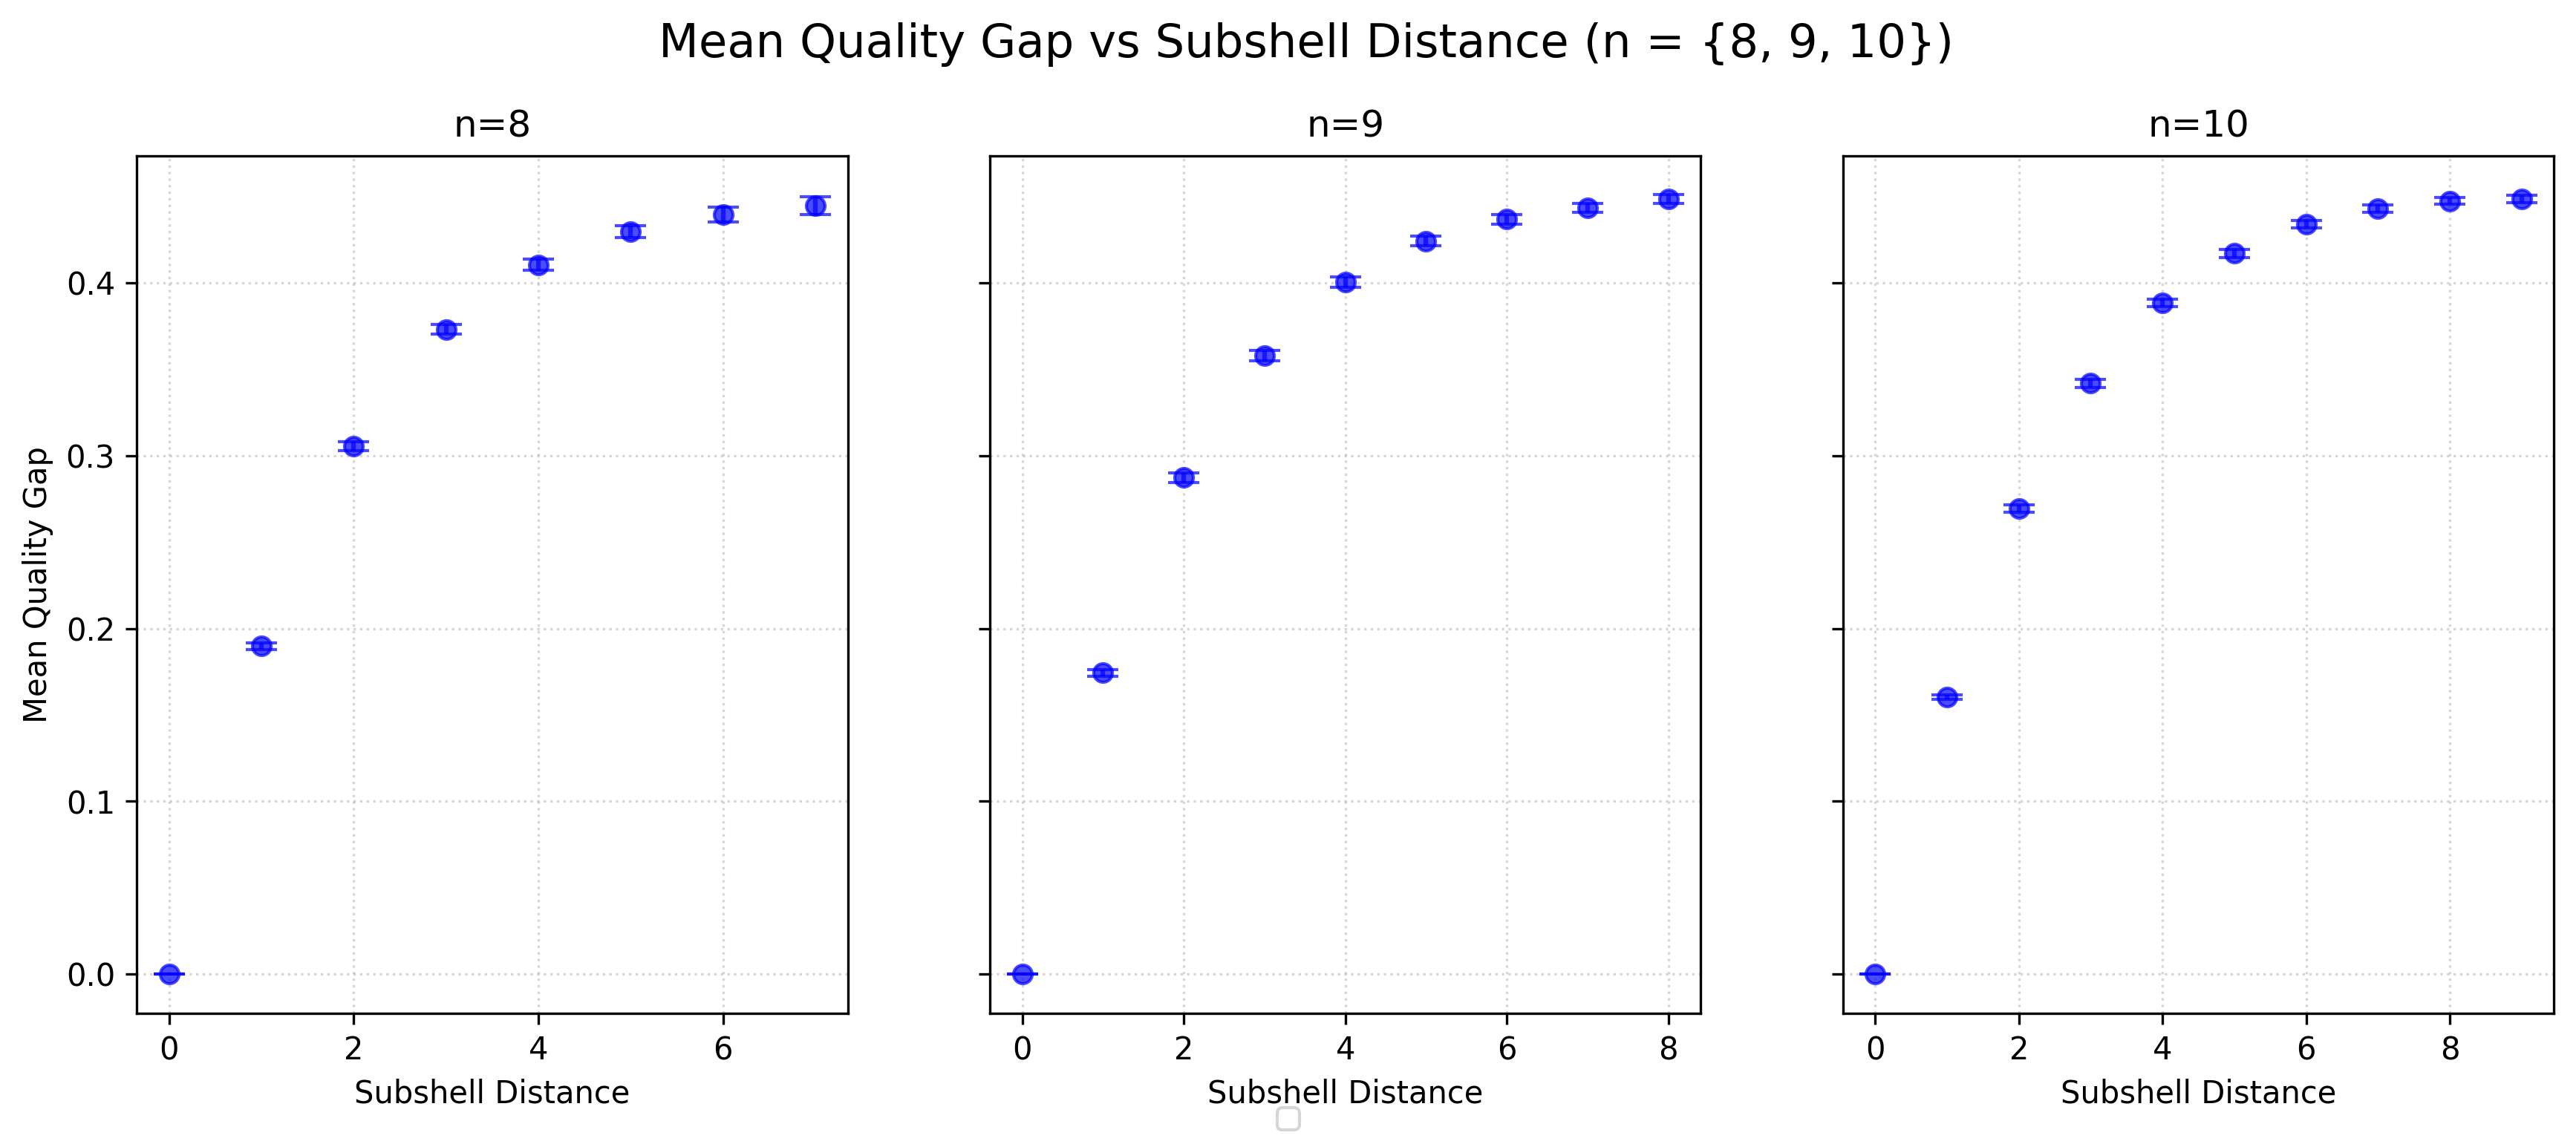
\includegraphics[width=\textwidth]{mean_quality_gap_vs_subshell_distance.png}
    \caption{Mean quality gap vs subshell distance}
    \label{fig:mqg}
\end{figure}

Figure \ref{fig:shell variance} shows the amount of variance in the objective values for each subshell.
Lower variance indicates more phase-coherence within the shell, and therefore more potential for constructive interference with the target solution under optimisation of $t$ and $\gamma$.
\begin{figure}[htbp]
    \centering
    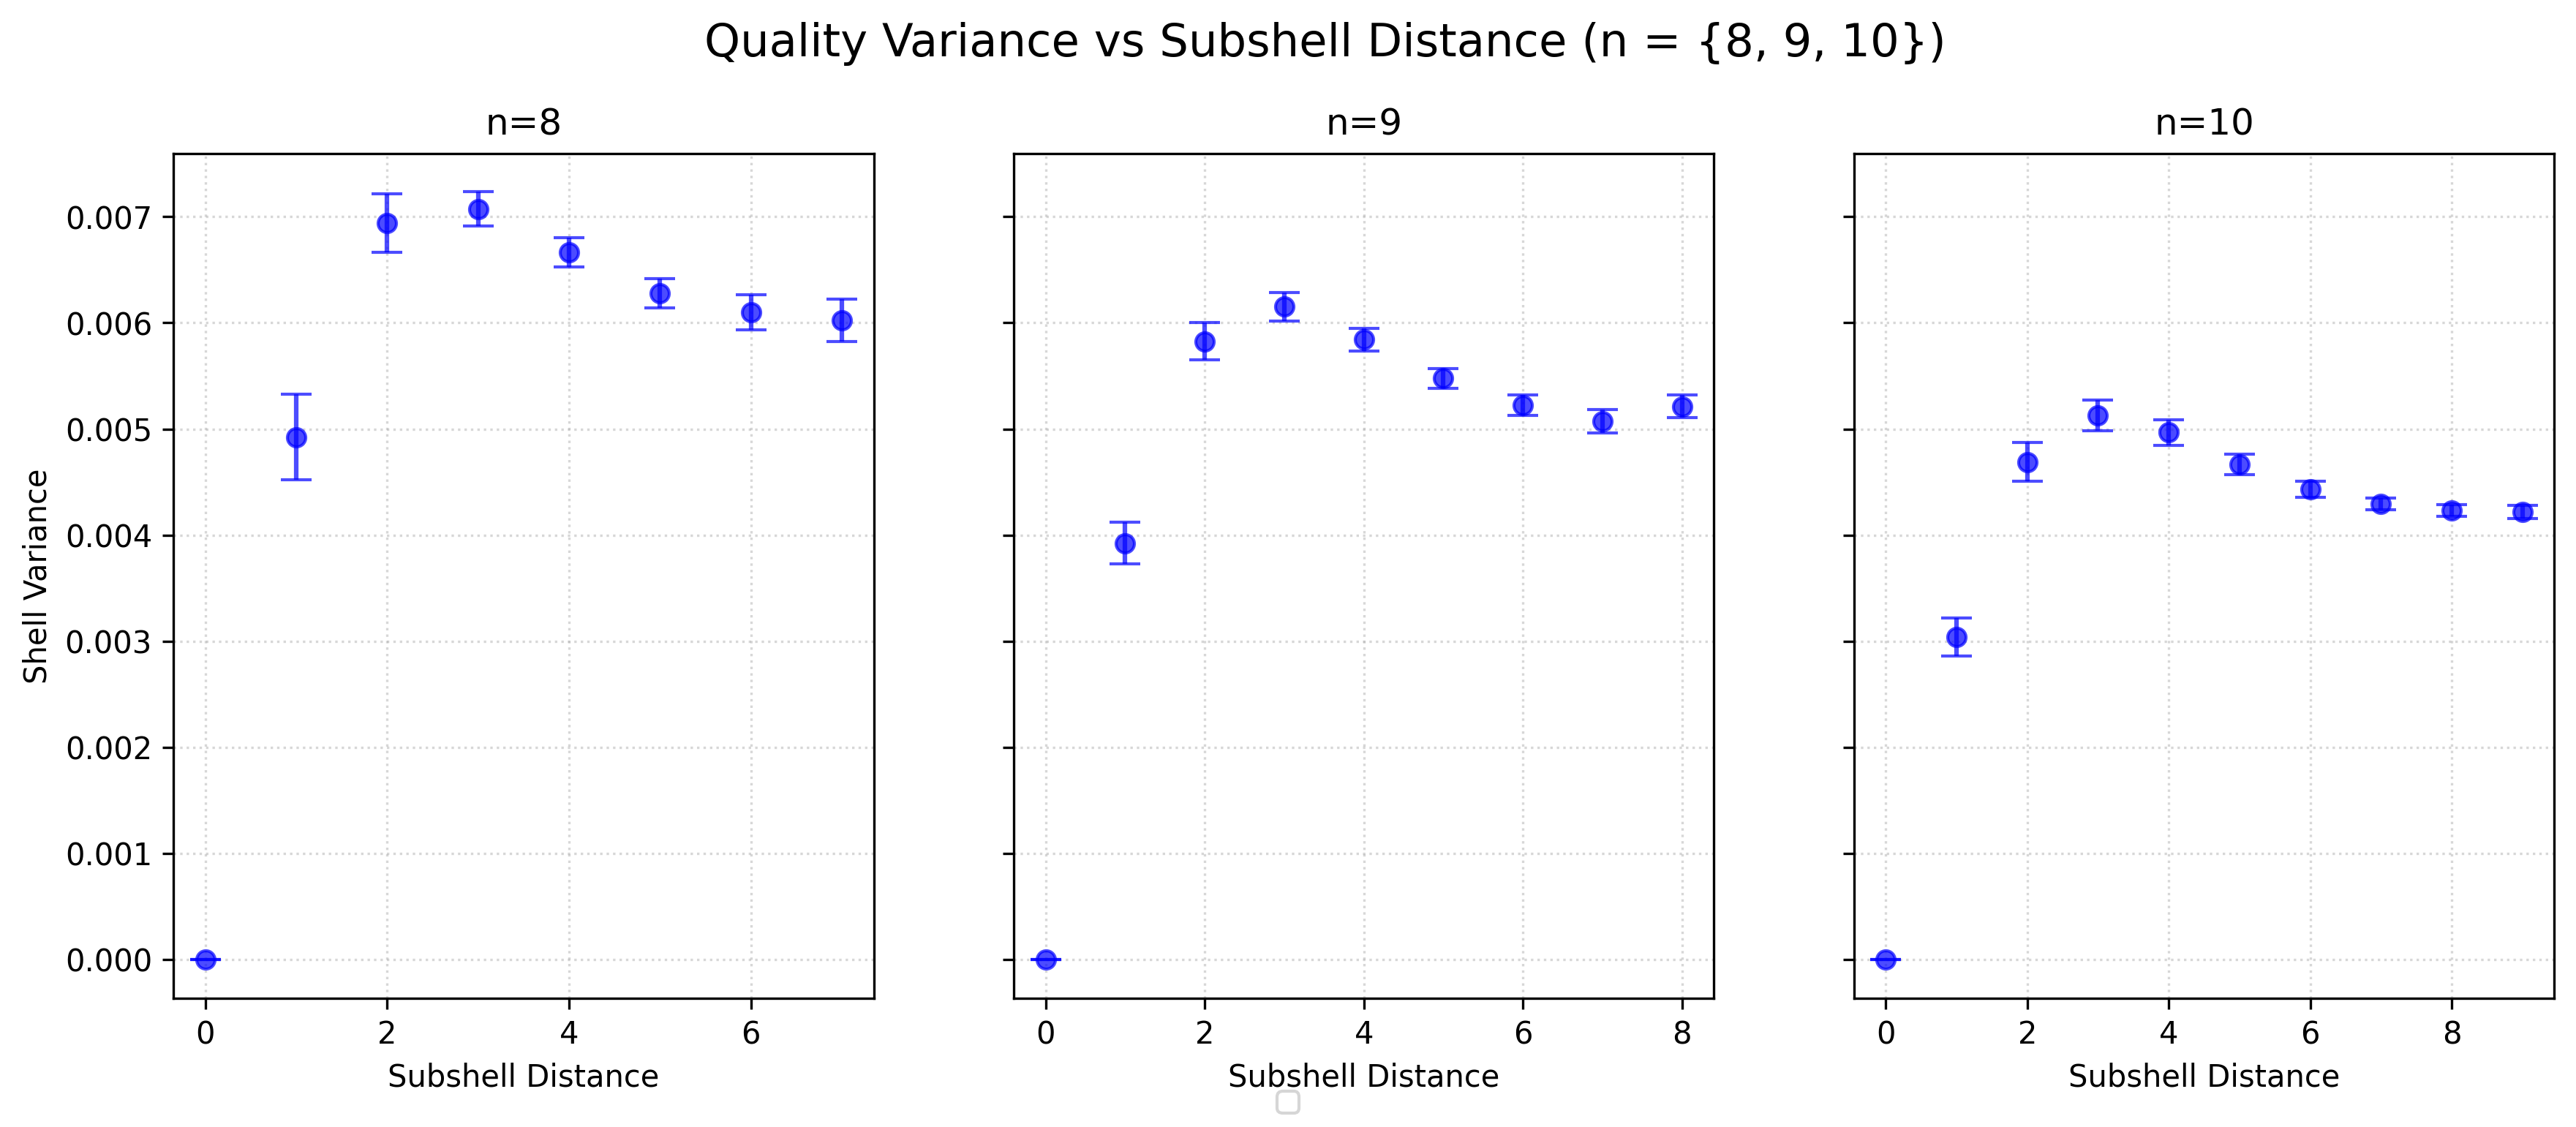
\includegraphics[width=\textwidth]{subshell_variance_multiple.png}
    \caption{Shell variance vs subshell distance}
    \label{fig:shell variance}
\end{figure}

\section{Hyperparameter Analysis}
Table of mean parameters:

\begin{tabular}{c|c|c|c}
    $n=8$          & $\beta$ & $\gamma$ & $t$     \\\hline
    Expected Value & 1.4(6)  & 0.20(4)  & 0.47(6) \\\hline
    OSP            & 0.79(5) & 1.00(4)  & 0.180(7)\\\hline
    CVaR           & 0.54(5) & 1.2(1)   & 0.17(1) 
\end{tabular}

\begin{tabular}{c|c|c|c}
    $n=9$          & $\beta$ & $\gamma$ & $t$     \\\hline
    Expected Value & 1.08(3) & 0.20(3)  & 0.40(6) \\\hline
    OSP            & 0.84(3) & 1.01(4)  & 0.164(7)\\\hline
    CVaR           & 0.60(3) & 1.16(9)  & 0.16(5) 
\end{tabular}

\begin{tabular}{c|c|c|c}
    $n=10$         & $\beta$ & $\gamma$ & $t$     \\\hline
    Expected Value & 1.10(3) & 0.21(2)  & 0.336(4)\\\hline
    OSP            & 0.85(7) & 1.02(5)  & 0.16(4) \\\hline
    CVaR           & 0.58(2) & 1.28(5)  & 0.124(6)
\end{tabular}
